\documentclass[11pt,a4paper]{article}
\usepackage[utf8]{inputenc}
\usepackage[T1]{fontenc}
\usepackage{lmodern}
\usepackage[brazil]{babel}
\usepackage[margin=2.3cm]{geometry}
\usepackage{amsmath,amssymb}
\usepackage{booktabs,array,graphicx,float,multirow}
\usepackage[table]{xcolor}
\usepackage{tcolorbox}
\usepackage{hyperref}
\hypersetup{colorlinks=true,linkcolor=blue!50!black}
\setlength{\parindent}{0pt}\setlength{\parskip}{5pt}
\newcommand{\Vc}[1]{V_{c#1}}
\newcommand{\Vin}{V_{in}}
\newcommand{\pct}{\,\%}
\newcommand{\num}[1]{\mathrm{#1}}
\newtcolorbox{just}{colback=blue!4,colframe=blue!50!black,title=Por que isso?,fonttitle=\bfseries\small,boxrule=.5pt,left=4pt,right=4pt,top=2pt,bottom=2pt}
\newtcolorbox{res}{colback=green!5,colframe=green!40!black,title=Resultado,fonttitle=\bfseries\small,boxrule=.5pt,left=4pt,right=4pt,top=2pt,bottom=2pt}
\newtcolorbox{formula}{colback=orange!6,colframe=orange!60!black,title=Fórmula de partida,fonttitle=\bfseries\small,boxrule=.5pt,left=4pt,right=4pt,top=2pt,bottom=2pt}
\newtcolorbox{todo}{colback=yellow!10,colframe=yellow!50!black,title=Experimento (a preencher na bancada),fonttitle=\bfseries\small,boxrule=.5pt,left=4pt,right=4pt,top=2pt,bottom=2pt}

\begin{document}
\begin{center}
{\LARGE\bfseries Segunda Avaliação de Controle de Processos}\\[4pt]
{\Large Resolução detalhada, com todos os cálculos por extenso (material de estudo)}\\[8pt]
Aluno(a): Izabella Camops Trarbach\\
Prof.\ Saul da S.\ Munareto --- Engenharia de Controle e Automação --- IFES Serra\\
Circuito G; planta de controle: $\Vc3/\Vin$
\end{center}

\begin{tcolorbox}[colback=gray!6,colframe=gray!60]
\textbf{Como ler este documento.} Cada cálculo segue sempre a mesma ordem:
\textbf{(1)} a fórmula padrão (caixa laranja); \textbf{(2)} a modificação necessária para o nosso caso, com a justificativa (caixa azul);
\textbf{(3)} a substituição dos números, passo a passo; \textbf{(4)} o resultado (caixa verde).
Todas as grandezas estão em \% da escala (100\,\% $=5$ V do Arduino), e os tempos em segundos.
Os números intermediários foram arredondados só na apresentação; todas as contas foram refeitas por computador sem arredondar e conferidas.
Os resultados experimentais de malha fechada (bancada) ficam nas caixas amarelas, a preencher depois dos ensaios.
Os dados brutos do ScadaBR (arquivo \texttt{Tiago\_Izabella\_260921.csv}) não estão neste documento: as tabelas que dependem deles (instantes de 28,3\,\% etc.\ e erros RMS contra o experimento) foram tiradas do relatório original.
\end{tcolorbox}

\tableofcontents
\newpage
%==================== PARTE 1 ====================
\section{O circuito e os valores medidos}
O circuito é de três estágios RC acoplados, com $R_4$ ligado ao terra:
\[
\Vin \;-\; R_1 \;-\; \underbrace{\Vc1}_{C_1} \;-\; R_2 \;-\; \underbrace{\Vc2}_{C_2} \;-\; R_3 \;-\; \underbrace{\Vc3}_{C_3} \;-\; R_4 \;-\; \text{terra}
\]
Valores medidos com o multímetro:
\begin{center}
\begin{tabular}{cccc|ccc}
\toprule $R_1$ & $R_2$ & $R_3$ & $R_4$ & $C_1$ & $C_2$ & $C_3$\\ \midrule
22,0 k$\Omega$ & 46,8 k$\Omega$ & 32,6 k$\Omega$ & 66,8 k$\Omega$ & 947 $\mu$F & 947 $\mu$F & 955 $\mu$F\\ \bottomrule
\end{tabular}
\end{center}

\subsection{Condutâncias}
\begin{formula}\[ g_k=\frac{1}{R_k} \]\end{formula}
\begin{just}Trabalhar com condutâncias evita frações aninhadas: a corrente num resistor é simplesmente $g\cdot\Delta V$.\end{just}
\begin{align*}
g_1&=\frac{1}{22\,000}=45{,}455\ \mu\mathrm{S}, & g_2&=\frac{1}{46\,800}=21{,}368\ \mu\mathrm{S},\\
g_3&=\frac{1}{32\,600}=30{,}675\ \mu\mathrm{S}, & g_4&=\frac{1}{66\,800}=14{,}970\ \mu\mathrm{S}.
\end{align*}
Somas que vão aparecer nas equações (cada nó soma as condutâncias dos dois resistores ligados a ele):
\begin{align*}
A_1&=g_1+g_2=45{,}455+21{,}368=66{,}822\ \mu\mathrm{S}\\
A_2&=g_2+g_3=21{,}368+30{,}675=52{,}042\ \mu\mathrm{S}\\
A_3&=g_3+g_4=30{,}675+14{,}970=45{,}645\ \mu\mathrm{S}
\end{align*}

%------------------------------------------------------------------
\section{Modelo matemático completo (funções de transferência da 1ª avaliação)}
\subsection{Equações dos nós (leis de Kirchhoff das correntes)}
\begin{formula}
Em cada nó: \emph{corrente que chega pelo resistor da esquerda = corrente que vai ao capacitor + corrente que sai pelo resistor da direita}, com $i_C=C\,\dfrac{dv}{dt}$ e $i_R=\dfrac{\Delta V}{R}$.
\end{formula}
\begin{align}
C_1\dot V_{c1}&=\frac{\Vin-\Vc1}{R_1}-\frac{\Vc1-\Vc2}{R_2}\\
C_2\dot V_{c2}&=\frac{\Vc1-\Vc2}{R_2}-\frac{\Vc2-\Vc3}{R_3}\\
C_3\dot V_{c3}&=\frac{\Vc2-\Vc3}{R_3}-\frac{\Vc3-0}{R_4}
\end{align}
\begin{just}O nó 3 só tem $R_4$ para o terra (por isso a tensão do terra é 0). Não existe um quarto capacitor: o sistema tem 3 estados ($\Vc1,\Vc2,\Vc3$), logo é de 3ª ordem.\end{just}

\subsection{Transformada de Laplace}
\begin{just}O circuito é linear e invariante no tempo. Trabalhando com desvios em torno de um ponto de operação (condições iniciais nulas), a derivada vira multiplicação por $s$: $\dot V\to sV$. Isso transforma o sistema diferencial num sistema algébrico.\end{just}
Substituindo $1/R_k=g_k$ e agrupando os termos de cada tensão:
\begin{align*}
(C_1s+g_1+g_2)\,\Vc1-g_2\,\Vc2&=g_1\,\Vin\\
-g_2\,\Vc1+(C_2s+g_2+g_3)\,\Vc2-g_3\,\Vc3&=0\\
-g_3\,\Vc2+(C_3s+g_3+g_4)\,\Vc3&=0
\end{align*}
Definindo $a_{11}=C_1s+A_1$, $a_{22}=C_2s+A_2$, $a_{33}=C_3s+A_3$, em forma matricial $M(s)\mathbf V=\mathbf b\,\Vin$:
\[
\begin{bmatrix}a_{11}&-g_2&0\\-g_2&a_{22}&-g_3\\0&-g_3&a_{33}\end{bmatrix}
\begin{bmatrix}\Vc1\\\Vc2\\\Vc3\end{bmatrix}=\begin{bmatrix}g_1\\0\\0\end{bmatrix}\Vin .
\]

\subsection{Determinante $\Delta(s)=\det M(s)$ (polinômio característico)}
Expansão pela primeira linha:
\[
\Delta=a_{11}\,(a_{22}a_{33}-g_3^2)-(-g_2)\big[(-g_2)a_{33}-(-g_3)\cdot0\big]=a_{11}\,(a_{22}a_{33}-g_3^2)-g_2^2\,a_{33}.
\]
Chamo $P(s)=a_{22}a_{33}-g_3^2$ e expando $(C_2s+A_2)(C_3s+A_3)=C_2C_3s^2+(C_2A_3+C_3A_2)s+A_2A_3$:
\[
P(s)=P_2s^2+P_1s+P_0,\quad P_2=C_2C_3,\;\; P_1=C_2A_3+C_3A_2,\;\; P_0=A_2A_3-g_3^2 .
\]
Substituindo os valores (capacitâncias em F, condutâncias em S):
\begin{align*}
P_2&=947\!\times\!10^{-6}\cdot955\!\times\!10^{-6}=9{,}044\times10^{-7}\\
P_1&=947\!\times\!10^{-6}\cdot45{,}645\!\times\!10^{-6}+955\!\times\!10^{-6}\cdot52{,}042\!\times\!10^{-6}\\&=4{,}323\times10^{-8}+4{,}970\times10^{-8}=9{,}293\times10^{-8}\\
P_0&=52{,}042\!\times\!10^{-6}\cdot45{,}645\!\times\!10^{-6}-(30{,}675\!\times\!10^{-6})^2\\&=2{,}3755\times10^{-9}-9{,}410\times10^{-10}=1{,}435\times10^{-9}
\end{align*}
Agora $\Delta=(C_1s+A_1)P(s)-g_2^2(C_3s+A_3)$. Multiplicando e agrupando por potências de $s$: $\Delta=D_3s^3+D_2s^2+D_1s+D_0$,
\begin{align*}
D_3&=C_1P_2=947\!\times\!10^{-6}\cdot9{,}044\!\times\!10^{-7}=8{,}565\times10^{-10}\\
D_2&=C_1P_1+A_1P_2=8{,}800\times10^{-11}+6{,}043\times10^{-11}=1{,}484\times10^{-10}\\
D_1&=C_1P_0+A_1P_1-g_2^2C_3=1{,}358\times10^{-12}+6{,}210\times10^{-12}-4{,}360\times10^{-13}=7{,}132\times10^{-12}\\
D_0&=A_1P_0-g_2^2A_3=9{,}586\times10^{-14}-2{,}084\times10^{-14}=7{,}502\times10^{-14}
\end{align*}
(onde $g_2^2=4{,}566\times10^{-10}\ \mathrm{S^2}$).

\subsection{Numeradores pela regra de Cramer}
\begin{formula}$V_{cj}=\Delta_j/\Delta$, onde $\Delta_j$ é o determinante de $M$ com a coluna $j$ trocada por $\mathbf b\Vin=[g_1\Vin\ 0\ 0]^T$.\end{formula}
\textbf{$\Vc3$ (coluna 3 trocada).} Expandindo pela terceira coluna (só o 1º elemento é não nulo):
\[
\Delta_3=g_1\Vin\det\begin{bmatrix}-g_2&a_{22}\\0&-g_3\end{bmatrix}=g_1\Vin\,(g_2g_3)\ \Rightarrow\ \frac{\Vc3}{\Vin}=\frac{g_1g_2g_3}{\Delta(s)}.
\]
\textbf{$\Vc2$ (coluna 2 trocada).} Só o 1º elemento é não nulo, com sinal $-1$ (posição (1,2)):
\[
\Delta_2=-g_1\Vin\det\begin{bmatrix}-g_2&-g_3\\0&a_{33}\end{bmatrix}=-g_1\Vin(-g_2a_{33})=g_1g_2a_{33}\Vin\ \Rightarrow\ \frac{\Vc2}{\Vin}=\frac{g_1g_2(C_3s+A_3)}{\Delta(s)}.
\]
\textbf{$\Vc1$ (coluna 1 trocada).} Expandindo pela primeira coluna:
\[
\Delta_1=g_1\Vin\det\begin{bmatrix}a_{22}&-g_3\\-g_3&a_{33}\end{bmatrix}=g_1\Vin\,P(s)\ \Rightarrow\ \frac{\Vc1}{\Vin}=\frac{g_1P(s)}{\Delta(s)}.
\]
\begin{just}Os três quocientes têm o \emph{mesmo denominador} $\Delta(s)$: é o polinômio característico da matriz, e por isso as três tensões compartilham os mesmos polos. O que muda é o numerador (os zeros).\end{just}

\subsection{Normalização (termo constante igual a 1)}
\begin{just}A forma padrão de função de transferência para processos é $K\,\dfrac{\prod(\tau_{z}s+1)}{\prod(\tau_{p}s+1)}$: o termo independente de $s$ vale 1, e o ganho estático $K$ aparece explicitamente. Para chegar lá, divido numerador e denominador por $D_0$ (o termo independente de $\Delta$).\end{just}
\[
\frac{\Delta}{D_0}=\frac{D_3}{D_0}s^3+\frac{D_2}{D_0}s^2+\frac{D_1}{D_0}s+1=\frac{8{,}565\times10^{-10}}{7{,}502\times10^{-14}}s^3+\frac{1{,}484\times10^{-10}}{7{,}502\times10^{-14}}s^2+\frac{7{,}132\times10^{-12}}{7{,}502\times10^{-14}}s+1
\]
\[
D(s)=11\,416{,}7\,s^3+1978{,}65\,s^2+95{,}071\,s+1 .
\]
\begin{res}
\[\frac{\Vc3}{\Vin}=\frac{0{,}3971}{11\,416{,}7\,s^3+1978{,}65\,s^2+95{,}071\,s+1}\]
\[\frac{\Vc2}{\Vin}=\frac{0{,}5910\,(20{,}92\,s+1)}{D(s)},\qquad \frac{\Vc1}{\Vin}=\frac{0{,}8692\,(630{,}4\,s^2+64{,}78\,s+1)}{D(s)}\]
\end{res}
Como os numeradores foram obtidos:
\begin{itemize}
\item $\Vc3$: $\dfrac{g_1g_2g_3}{D_0}=\dfrac{45{,}455\cdot21{,}368\cdot30{,}675\times10^{-18}}{7{,}502\times10^{-14}}=\dfrac{2{,}979\times10^{-14}}{7{,}502\times10^{-14}}=0{,}3971$.
\item $\Vc2$: $\dfrac{g_1g_2(C_3s+A_3)}{D_0}=\dfrac{g_1g_2A_3}{D_0}\left(\dfrac{C_3}{A_3}s+1\right)$; $\dfrac{g_1g_2A_3}{D_0}=\dfrac{4{,}433\times10^{-14}}{7{,}502\times10^{-14}}=0{,}5910$ e $\dfrac{C_3}{A_3}=\dfrac{955\times10^{-6}}{45{,}645\times10^{-6}}=20{,}92$ s.
\item $\Vc1$: $\dfrac{g_1P(s)}{D_0}=\dfrac{g_1P_0}{D_0}\left(\dfrac{P_1}{P_0}s+\dfrac{P_2}{P_0}s^2+1\right)$; $\dfrac{g_1P_0}{D_0}=\dfrac{6{,}520\times10^{-14}}{7{,}502\times10^{-14}}=0{,}8692$, $\dfrac{P_1}{P_0}=\dfrac{9{,}293\times10^{-8}}{1{,}435\times10^{-9}}=64{,}78$, $\dfrac{P_2}{P_0}=\dfrac{9{,}044\times10^{-7}}{1{,}435\times10^{-9}}=630{,}4$.
\end{itemize}

\subsection{Ganhos estáticos (duas conferências)}
O ganho estático é $G(0)$. Pelo método anterior: $K_3=0{,}3971$, $K_2=0{,}5910$, $K_1=0{,}8692$.

\textbf{Conferência por divisores resistivos.} Em regime permanente os capacitores são circuitos abertos (corrente nula), então a mesma corrente $\Vin/R_t$ percorre todos os resistores, com $R_t=R_1+R_2+R_3+R_4=22+46{,}8+32{,}6+66{,}8=168{,}2$ k$\Omega$:
\[\begin{gathered}
K_3=\frac{R_4}{R_t}=\frac{66{,}8}{168{,}2}=0{,}3971,\\
K_2=\frac{R_3+R_4}{R_t}=\frac{99{,}4}{168{,}2}=0{,}5910,\\
K_1=\frac{R_2+R_3+R_4}{R_t}=\frac{146{,}2}{168{,}2}=0{,}8692 .
\end{gathered}\]
Os dois caminhos coincidem, o que confirma o modelo.

\subsection{Polos, zeros e constantes de tempo}
As raízes de $D(s)=0$ (cúbica, resolvida numericamente) são
$s_1=-0{,}01456$, $s_2=-0{,}06250$, $s_3=-0{,}09625$ s$^{-1}$.
\begin{formula}Cada polo real $s=-1/\tau_i$ dá uma constante de tempo $\tau_i=-1/s$; o denominador fatora em $(\tau_1s+1)(\tau_2s+1)(\tau_3s+1)$.\end{formula}
\[
\tau_1=\frac{1}{0{,}01456}=68{,}68\ \mathrm{s},\qquad \tau_2=\frac{1}{0{,}06250}=16{,}00\ \mathrm{s},\qquad \tau_3=\frac{1}{0{,}09625}=10{,}39\ \mathrm{s}.
\]
\textbf{Verificação pelas relações de Vieta} (coeficientes do produto $(\tau_1s+1)(\tau_2s+1)(\tau_3s+1)$ devem ser os de $D(s)$):
\begin{align*}
\tau_1+\tau_2+\tau_3&=68{,}68+16{,}00+10{,}39=95{,}07\ \ \checkmark\ (\text{coef. de }s)\\
\tau_1\tau_2+\tau_1\tau_3+\tau_2\tau_3&=1098{,}9+713{,}6+166{,}2=1978{,}7\ \ \checkmark\ (\text{coef. de }s^2)\\
\tau_1\tau_2\tau_3&=68{,}68\cdot16{,}00\cdot10{,}39=11\,416{,}7\ \ \checkmark\ (\text{coef. de }s^3)
\end{align*}
Todas as raízes são reais e negativas $\Rightarrow$ sistema estável e \textbf{sobreamortecido} (sem oscilação). A constante \emph{dominante} é $\tau_1=68{,}68$ s (a maior; é $68{,}68/16{,}00=4{,}29$ vezes a segunda).

\textbf{Zeros (constantes de tempo de avanço):}
\begin{itemize}
\item $\Vc3$: o numerador é constante $\Rightarrow$ não há zeros.
\item $\Vc2$: o zero é a raiz de $C_3s+A_3=0$, isto é, $\tau_z=C_3/A_3=20{,}92$ s.
\item $\Vc1$: os zeros são as raízes de $630{,}4s^2+64{,}78s+1=0$. Por Bhaskara:
\[
\Delta=64{,}78^2-4\cdot630{,}4\cdot1=4196{,}4-2521{,}6=1674{,}8,\quad\sqrt\Delta=40{,}92,
\]
\[
s=\frac{-64{,}78\pm40{,}92}{2\cdot630{,}4}\ \Rightarrow\ s_{z1}=-0{,}01892,\ s_{z2}=-0{,}08383\ \Rightarrow\ \tau_{z1}=52{,}85\ \mathrm{s},\ \tau_{z2}=11{,}93\ \mathrm{s}.
\]
Conferência: $52{,}85\cdot11{,}93=630{,}5$ e $52{,}85+11{,}93=64{,}78$ $\checkmark$.
\end{itemize}
\begin{res}
\begin{align}
\frac{\Vc3}{\Vin}&=\frac{0{,}3971}{(68{,}68s+1)(16{,}00s+1)(10{,}39s+1)}\label{ft3}\\
\frac{\Vc2}{\Vin}&=\frac{0{,}5910\,(20{,}92s+1)}{(68{,}68s+1)(16{,}00s+1)(10{,}39s+1)}\\
\frac{\Vc1}{\Vin}&=\frac{0{,}8692\,(52{,}85s+1)(11{,}93s+1)}{(68{,}68s+1)(16{,}00s+1)(10{,}39s+1)}
\end{align}
\end{res}
\begin{just}\textbf{Tipo de curva previsto pelo grau relativo} (polos $-$ zeros): $\Vc1$ tem $3-2=1$, então a derivada em $t=0^+$ é diferente de zero e a curva tem inclinação máxima logo no início (\textbf{curva tipo C}). $\Vc2$ tem $3-1=2$ e $\Vc3$ tem $3-0=3$: a inclinação inicial é nula e há ponto de inflexão (\textbf{curva tipo S}). Isso diz de antemão qual método de redução usar em cada tensão. O sistema é \emph{interativo}: as constantes de tempo (10,4; 16,0; 68,7 s) são bem diferentes das de cada estágio isolado ($R_1C_1=20{,}8$ s etc.), porque cada capacitor carrega e descarrega os vizinhos.\end{just}

\subsection{Resposta ao degrau da FT completa (frações parciais)}
\begin{formula}Para $u=U\cdot1(t)$ e $G(s)=K\dfrac{\prod_k(\tau_{z,k}s+1)}{\prod_i(\tau_is+1)}$ com polos distintos:
\[
y(t)=K\Big[1-\sum_{i=1}^{3}c_i\,e^{-t/\tau_i}\Big],\qquad c_i=\frac{\prod_k\left(1-\tau_{z,k}/\tau_i\right)}{\prod_{j\ne i}\left(1-\tau_j/\tau_i\right)}\quad(U=1).\]
\end{formula}
\begin{just}O resíduo da exponencial em $s=-1/\tau_i$ é obtido multiplicando $Y(s)$ por $(\tau_is+1)$ e calculando em $s=-1/\tau_i$. Em $s=0$ o resíduo é $K$ (valor final). Como $y(0)=0$, deve valer $\sum c_i=1$ --- é a conferência.\end{just}
Exemplo detalhado: $\Vc3$, $c_1$ (polo $\tau_1=68{,}68$):
\[
c_1=\frac{1}{(1-\tau_2/\tau_1)(1-\tau_3/\tau_1)}=\frac{1}{(1-0{,}2329)(1-0{,}1513)}=\frac{1}{0{,}7671\cdot0{,}8487}=1{,}536 .
\]
Exemplo $\Vc2$, $c_1$ (numerador com $\tau_z=20{,}92$): $c_1=\dfrac{1-20{,}92/68{,}68}{0{,}7671\cdot0{,}8487}=\dfrac{0{,}6954}{0{,}6510}=1{,}068$. Os demais coeficientes seguem o mesmo procedimento:
\begin{center}
\begin{tabular}{lccc}\toprule & $c_1$ ($\tau_1=68{,}7$) & $c_2$ ($\tau_2=16{,}0$) & $c_3$ ($\tau_3=10{,}4$)\\\midrule
$\Vc3$ & $1{,}5360$ & $-0{,}8662$ & $0{,}3302$\\ $\Vc2$ & $1{,}0681$ & $0{,}2666$ & $-0{,}3347$\\ $\Vc1$ & $0{,}2926$ & $0{,}5075$ & $0{,}1999$\\\bottomrule
\end{tabular}
\end{center}
Conferência $\sum c_i=1$ em cada linha (p.\,ex.\ $\Vc3$: $1{,}5360-0{,}8662+0{,}3302=1{,}0000$). Esta expressão é a ``resposta da FT completa'' usada nas comparações.

%------------------------------------------------------------------
\section{Teste ao degrau experimental}
\subsection{O arquivo e o trecho usado}
O ScadaBR gravou uma amostra por segundo de cinco variáveis (1440 amostras cada): $SO=\Vin$, $VP=\Vc3$, $VP1=\Vc2$, $VP2=\Vc1$ (e $SP$). A entrada \texttt{SO} fica em 30\,\% nos primeiros 41 s, em 70\,\% até $t=577$ s e depois em 50\,\% até o fim. Para identificar as FTs reduzidas usei \textbf{apenas o degrau de 70\,\% para 50\,\%}:
\[
\Delta U=U_1-U_0=50{,}000-70{,}001=-20{,}000\,\%\ (\approx-1\ \mathrm{V}),\qquad t_{degrau}=576{,}5\ \mathrm{s}.
\]
\begin{just}O degrau começa de um regime permanente real (o patamar de 70\,\% dura 535 s, mais de $7\tau_1=481$ s) e termina em outro patamar longo (863 s). Assim $y_i$ e $y_f$ são confiáveis e não há transitório de teste anterior contaminando. Como o circuito é linear, o resultado vale para qualquer ponto de operação e para degraus em qualquer sentido.\end{just}
\begin{figure}[H]\centering
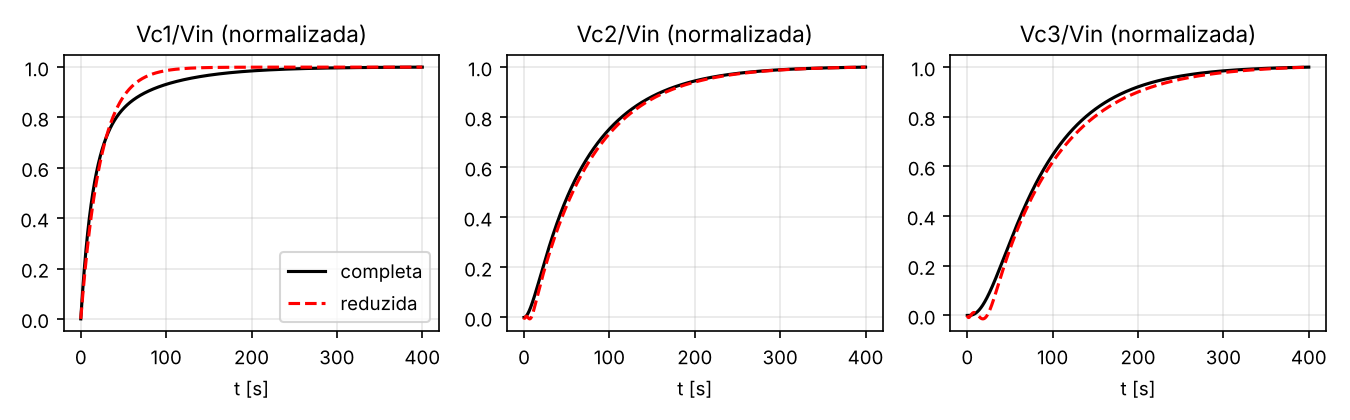
\includegraphics[width=.8\textwidth]{figs/steps.png}
\caption{Respostas ao degrau normalizadas das FTs completas (preto) e das reduzidas (vermelho tracejado), calculadas neste documento.}\end{figure}

\subsection{Tratamento dos dados}
\begin{formula}
$\displaystyle y_n(t)=\frac{y(t)-y_i}{y_f-y_i}$ (resposta normalizada, vai de 0 a 1);\qquad $\displaystyle K=\frac{y_f-y_i}{\Delta U}$.
\end{formula}
\begin{just}Normalizar elimina o sinal negativo do degrau (queda de 70 para 50) e permite aplicar as fórmulas dos métodos como se fosse um degrau positivo unitário. $y_i$ é a média das 128 amostras antes do degrau; $y_f$, a média das 150 últimas amostras (médias reduzem o ruído de quantização do ADC de 10 bits, resolução $100/1024=0{,}0977\,\%$).\end{just}
\begin{center}
\begin{tabular}{lccc}\toprule & $\Vc1$ & $\Vc2$ & $\Vc3$\\\midrule
$y_i$ [\%] (SO=70\,\%) & 60,774 & 41,104 & 27,454\\
$y_f$ [\%] (SO=50\,\%) & 43,431 & 29,382 & 19,618\\
$y_f-y_i$ [\%] & $-17{,}343$ & $-11{,}723$ & $-7{,}836$\\\bottomrule
\end{tabular}
\end{center}
\[
K_1=\frac{-17{,}343}{-20}=0{,}8671,\qquad K_2=\frac{-11{,}723}{-20}=0{,}5861,\qquad K_3=\frac{-7{,}836}{-20}=0{,}3918 .
\]
\textbf{Conferência pelo patamar final:} $y_f/50$: $43{,}431/50=0{,}8686$; $29{,}382/50=0{,}5876$; $19{,}618/50=0{,}3924$ (praticamente iguais, confirmando linearidade: saída nula para entrada nula).
\textbf{Comparação com a teoria:} o ganho medido fica 0,2\,\% a 1,3\,\% abaixo ($0{,}8671$ vs.\ $0{,}8692$; $0{,}5861$ vs.\ $0{,}5910$; $0{,}3918$ vs.\ $0{,}3971$), coerente com as tolerâncias dos $R$ e $C$, a quantização do ADC e a resistência de saída do Arduino. Adoto $K=(y_f-y_i)/\Delta U$, de modo que a FT reduzida termina exatamente no valor final medido.

\subsection{Instantes de 28,3\,\%, 35,3\,\%, 63,2\,\% e 85,3\,\%}
\begin{formula}Para cada nível $q$, procuro a primeira amostra $k+1$ com $y_n\ge q$ e interpolo linearmente entre $k$ e $k+1$:
\[t_q=t_k+\frac{q-y_{n,k}}{y_{n,k+1}-y_{n,k}}(t_{k+1}-t_k).\]\end{formula}
Exemplo completo ($\Vc3$, $q=0{,}632$): $t_k=103{,}5$ s ($y_{n,k}=0{,}6264$) e $t_{k+1}=104{,}5$ s ($y_{n,k+1}=0{,}6388$):
\[
t_{63,2}=103{,}5+\frac{0{,}632-0{,}6264}{0{,}6388-0{,}6264}\,(104{,}5-103{,}5)=103{,}5+\frac{0{,}0056}{0{,}0124}\cdot1=103{,}5+0{,}45=103{,}95\ \mathrm{s}.
\]
Resultados (em segundos desde o degrau):
\begin{center}
\begin{tabular}{lcccc}\toprule & $t_{28,3}$ & $t_{35,3}$ & $t_{63,2}$ & $t_{85,3}$\\\midrule
$\Vc1$ & 7,16 & 9,31 & 23,31 & 58,39\\ $\Vc2$ & 32,34 & 39,12 & 78,26 & 146,80\\ $\Vc3$ & 51,93 & 60,55 & 103,95 & 173,70\\\bottomrule
\end{tabular}
\end{center}

%------------------------------------------------------------------
\section{Redução a ganho, constante de tempo e atraso}
\subsection{O modelo reduzido e a origem dos métodos}
\begin{formula}Modelo de 1ª ordem com atraso (FOPDT): $\displaystyle G(s)=\frac{K\,e^{-t_0s}}{\tau s+1}$. Sua resposta ao degrau é $y_n(t)=1-e^{-(t-t_0)/\tau}$ para $t\ge t_0$ (e $0$ antes).\end{formula}
Cada método de identificação vem de impor que essa curva passe por pontos da curva real. Vou deduzir as constantes numéricas para entender de onde saem.

\textbf{Curva tipo C} (sem inflexão, inclinação máxima na origem; caso de $\Vc1$): não há atraso, $t_0=0$, e em $t=\tau$ a resposta vale $1-e^{-1}=0{,}632$. Logo $\tau=t_{63,2}$.

\textbf{Curva tipo S, método de Smith (Ajuste 3, seção 7-2.1 do livro).} Impondo que a FOPDT passe pelos pontos de 28,3\,\% e 63,2\,\%:
\[\begin{gathered}
1-e^{-(t_{28,3}-t_0)/\tau}=0{,}283\ \Rightarrow\ \frac{t_{28,3}-t_0}{\tau}=-\ln(0{,}717)=0{,}333\approx\frac13,\\
1-e^{-(t_{63,2}-t_0)/\tau}=0{,}632\ \Rightarrow\ \frac{t_{63,2}-t_0}{\tau}=1 .
\end{gathered}\]
Subtraindo: $t_{63,2}-t_{28,3}=\tau(1-\tfrac13)=\tfrac23\tau$. Logo
\[
\boxed{\tau=1{,}5\,(t_{63,2}-t_{28,3}),\qquad t_0=t_{63,2}-\tau .}
\]
\textbf{Método de Sundaresan--Krishnaswamy} (mesmo raciocínio com 35,3\,\% e 85,3\,\%):
$\frac{t_{35,3}-t_0}{\tau}=-\ln(0{,}647)=0{,}435$ e $\frac{t_{85,3}-t_0}{\tau}=-\ln(0{,}147)=1{,}917$. Subtraindo: $t_{85,3}-t_{35,3}=1{,}482\tau$, logo $\tau=0{,}675\,(t_{85,3}-t_{35,3})\approx0{,}67(t_{85,3}-t_{35,3})$ e $t_0=t_{35,3}-0{,}435\tau=1{,}3\,t_{35,3}-0{,}29\,t_{85,3}$.

\textbf{Método da tangente no ponto de inflexão (Ziegler--Nichols, Ajuste 1).} Acho o ponto de maior inclinação $(t_i,y_i)$ com inclinação $m$. A reta tangente $y=y_i+m(t-t_i)$ corta o eixo do tempo ($y=0$) em $t_0=t_i-y_i/m$ e atinge o valor final ($y=1$) em $t=t_i+(1-y_i)/m$; então $\tau=\big[t_i+(1-y_i)/m\big]-t_0$.

\subsection{Contas, passo a passo}
\textbf{$\Vc1$ (tipo C).} A inclinação máxima ocorre na primeira amostra ($m=0{,}0500$ s$^{-1}$; a derivada teórica em $0^+$ é $0{,}048$ s$^{-1}$, ver Lista 2). Então $t_0=0$ e $\tau=t_{63,2}=23{,}31$ s. \emph{Teste de coerência:} se eu tentasse Smith, $\tau=1{,}5(23{,}31-7{,}16)=24{,}23$ s e $t_0=23{,}31-24{,}23=-0{,}92$ s: atraso \emph{negativo}, sem sentido físico (a saída não antecipa a entrada), o que confirma que não há atraso.

\textbf{$\Vc2$ (tipo S), Smith:}
\[
\tau=1{,}5\,(78{,}26-32{,}34)=1{,}5\cdot45{,}92=68{,}88\ \mathrm{s},\qquad t_0=78{,}26-68{,}88=9{,}38\ \mathrm{s}.
\]
\textbf{$\Vc3$ (tipo S), Smith:}
\[
\tau=1{,}5\,(103{,}95-51{,}93)=1{,}5\cdot52{,}02=78{,}03\ \mathrm{s},\qquad t_0=103{,}95-78{,}03=25{,}92\ \mathrm{s}.
\]
\textbf{Sundaresan:} $\Vc2$: $\tau=0{,}67(146{,}80-39{,}12)=72{,}15$ s, $t_0=1{,}3\cdot39{,}12-0{,}29\cdot146{,}80=50{,}86-42{,}57=8{,}29$ s. $\Vc3$: $\tau=0{,}67(173{,}70-60{,}55)=75{,}81$ s, $t_0=1{,}3\cdot60{,}55-0{,}29\cdot173{,}70=78{,}72-50{,}37=28{,}35$ s.

\textbf{Tangente} (pontos de inflexão medidos): $\Vc2$: $t_i=22{,}5$, $y_i=0{,}178$, $m=0{,}01151$ s$^{-1}$: $t_0=22{,}5-0{,}178/0{,}01151=7{,}07$ s; $\tau=\big[22{,}5+(1-0{,}178)/0{,}01151\big]-7{,}07=93{,}93-7{,}07=86{,}86$ s. $\Vc3$: $t_i=43{,}5$, $y_i=0{,}213$, $m=0{,}00884$: $t_0=43{,}5-24{,}10=19{,}38$ s; $\tau=\big[43{,}5+0{,}787/0{,}00884\big]-19{,}38=132{,}5-19{,}38=113{,}10$ s.

\subsection{Resultados e escolha do método}
\begin{center}\small
\begin{tabular}{lccc}\toprule $\tau/t_0$ [s] & $\Vc1$ & $\Vc2$ & $\Vc3$\\\midrule
Tipo C ($\tau=t_{63,2}$, $t_0=0$) & \textbf{23,3 / 0,0} & 78,3 / 0,0 & 104,0 / 0,0\\
Smith (28,3/63,2) & 24,2 / $-0{,}9$ & \textbf{68,9 / 9,4} & \textbf{78,0 / 25,9}\\
Sundaresan (35,3/85,3) & 32,9 / $-4{,}8$ & 72,1 / 8,3 & 75,8 / 28,3\\
Tangente (Z--N) & 20,0 / 0,6 & 86,9 / 7,1 & 113,1 / 19,4\\
Mínimos quadrados (referência) & 27,0 / 0,0 & 72,1 / 7,5 & 79,7 / 23,4\\\bottomrule
\end{tabular}\end{center}
Para comparar os modelos com o experimento uso o erro RMS e o erro máximo, em \% do degrau:
\[
\begin{gathered}\varepsilon_{rms}=100\sqrt{\frac1N\sum_{k=1}^{N}\big(y_{mod,n}(t_k)-y_{exp,n}(t_k)\big)^2},\\
\varepsilon_{max}=100\max_k|y_{mod,n}(t_k)-y_{exp,n}(t_k)|,\quad 0<t<520\,\mathrm{s}\ (N=520).\end{gathered}
\]
RMS (máximo), vindos do relatório original com os dados:
\begin{center}\small
\begin{tabular}{lccc}\toprule & $\Vc1$ & $\Vc2$ & $\Vc3$\\\midrule
Tipo C & 2,87 (7,3) & 1,89 (8,5) & 4,89 (15,6)\\
Smith & 2,71 (6,8) & 0,71 (4,1) & 1,12 (7,1)\\
Sundaresan & 3,28 (13,3) & 0,53 (3,2) & 1,45 (9,1)\\
Tangente & 3,67 (9,4) & 3,55 (7,5) & 6,71 (12,6)\\
Mínimos quadrados & 2,48 (7,2) & 0,44 (2,6) & 0,97 (5,3)\\
FT completa & 0,73 (3,5) & 1,48 (3,2) & 1,75 (3,6)\\\bottomrule
\end{tabular}\end{center}
\begin{just}\textbf{$\Vc1$:} é curva tipo C (Smith dá atraso negativo), logo $\tau=t_{63,2}$ e $t_0=0$. \textbf{$\Vc2$ e $\Vc3$:} adoto Smith porque (i) é o método do livro (Ajuste 3); (ii) usa dois pontos no meio da subida, pouco sensíveis à quantização e ao valor final; (iii) seu erro RMS fica próximo ao dos mínimos quadrados (o melhor possível para uma FOPDT). A tangente é a pior (RMS 6,7\,\% em $\Vc3$): a inclinação máxima de um sistema de 3ª ordem é muito sensível à suavização dos dados. Tratar $\Vc3$ como curva C (RMS 4,9\,\%) também é ruim, o que confirma que ela é do tipo S.\end{just}
\textbf{Conferência independente (regra prática do livro, p.\,216):} $\tau\approx$ maior constante de tempo, $t_0\approx$ soma das menores. Com a Seção 2: $\tau\approx68{,}7$ s e $t_0\approx16{,}0+10{,}4=26{,}4$ s, próximo do identificado para $\Vc3$ ($78{,}0$ s e $25{,}9$ s).
\begin{res}
\[
\frac{\Vc1}{\Vin}\approx\frac{0{,}867}{23{,}3s+1},\qquad
\frac{\Vc2}{\Vin}\approx\frac{0{,}586\,e^{-9{,}4s}}{68{,}9s+1},\qquad
\frac{\Vc3}{\Vin}\approx\frac{0{,}392\,e^{-25{,}9s}}{78{,}0s+1}\ \ \text{(a planta de controle)}
\]
\end{res}

%------------------------------------------------------------------
\section{Comparação das respostas ao degrau}
A figura da Seção 3 já mostra as respostas normalizadas; os erros RMS acima quantificam: a FT completa acompanha o experimento com RMS de 0,7\,\% a 1,7\,\% do degrau (valida o modelo físico e as medidas de $R$ e $C$); a reduzida erra mais (2,9\,\% em $\Vc1$, 0,7\,\% em $\Vc2$, 1,1\,\% em $\Vc3$), o que é esperado: troca 3 polos (e zeros) por 1 polo e 1 atraso. Em $\Vc3$ e $\Vc2$ a reduzida reproduz o atraso inicial e a subida; a maior diferença está na cauda, pois o 1º ordem não representa o peso diferente do polo lento ($\tau_1=68{,}7$ s). Em $\Vc1$ a reduzida fica próxima da curva real até $\sim$20 s, cruza e depois fica acima, porque $\Vc1$ não é naturalmente de 1ª ordem (tem 3 polos e 2 zeros).

%------------------------------------------------------------------
\section{Diagramas de Bode e margens}
\subsection{Respostas em frequência}
\begin{formula}Substituindo $s=j\omega$ em $G(s)=K\prod(\tau_{z}s+1)/\prod(\tau_ps+1)$ e $G_{red}=Ke^{-t_0s}/(\tau s+1)$:
\[
|G_{compl}(j\omega)|=K\frac{\prod_k\sqrt{1+(\omega\tau_{z,k})^2}}{\prod_i\sqrt{1+(\omega\tau_i)^2}},\qquad
\angle G_{compl}=\sum_k\arctan(\omega\tau_{z,k})-\sum_i\arctan(\omega\tau_i),
\]
\[
|G_{red}(j\omega)|=\frac{K}{\sqrt{1+(\omega\tau)^2}},\qquad\angle G_{red}=-\arctan(\omega\tau)-\omega t_0\ (\text{rad}).
\]\end{formula}
\begin{just}O módulo de $(\tau s+1)$ em $s=j\omega$ é $\sqrt{1+\omega^2\tau^2}$ e sua fase é $\arctan(\omega\tau)$; polos entram no denominador (subtraem fase), zeros no numerador (somam fase). O atraso puro $e^{-j\omega t_0}$ tem módulo 1 e fase $-\omega t_0$, que decresce sem limite com $\omega$ --- por isso a FOPDT difere tanto da completa em alta frequência.\end{just}
\textbf{Exemplo numérico completo: $\Vc3$ em $\omega=0{,}1$ rad/s.} FT completa:
\begin{align*}
\sqrt{1+(0{,}1\cdot68{,}68)^2}&=\sqrt{1+47{,}17}=6{,}941, & \arctan(6{,}868)&=81{,}72^\circ\\
\sqrt{1+(0{,}1\cdot16{,}00)^2}&=\sqrt{1+2{,}56}=1{,}887, & \arctan(1{,}600)&=57{,}99^\circ\\
\sqrt{1+(0{,}1\cdot10{,}39)^2}&=\sqrt{1+1{,}079}=1{,}442, & \arctan(1{,}039)&=46{,}10^\circ
\end{align*}
\[
|G|=\frac{0{,}3971}{6{,}941\cdot1{,}887\cdot1{,}442}=\frac{0{,}3971}{18{,}89}=0{,}0210,\qquad \angle G=-(81{,}72+57{,}99+46{,}10)=-185{,}8^\circ .
\]
FT reduzida: $\sqrt{1+(0{,}1\cdot78{,}03)^2}=\sqrt{1+60{,}89}=7{,}867$, $|G|=0{,}3918/7{,}867=0{,}0498$; fase $=-\arctan(7{,}803)-0{,}1\cdot25{,}92\ \mathrm{rad}=-82{,}70^\circ-148{,}52^\circ=-231{,}2^\circ$ (o atraso contribui com $\omega t_0=2{,}592\ \mathrm{rad}=148{,}5^\circ$).

\begin{figure}[H]\centering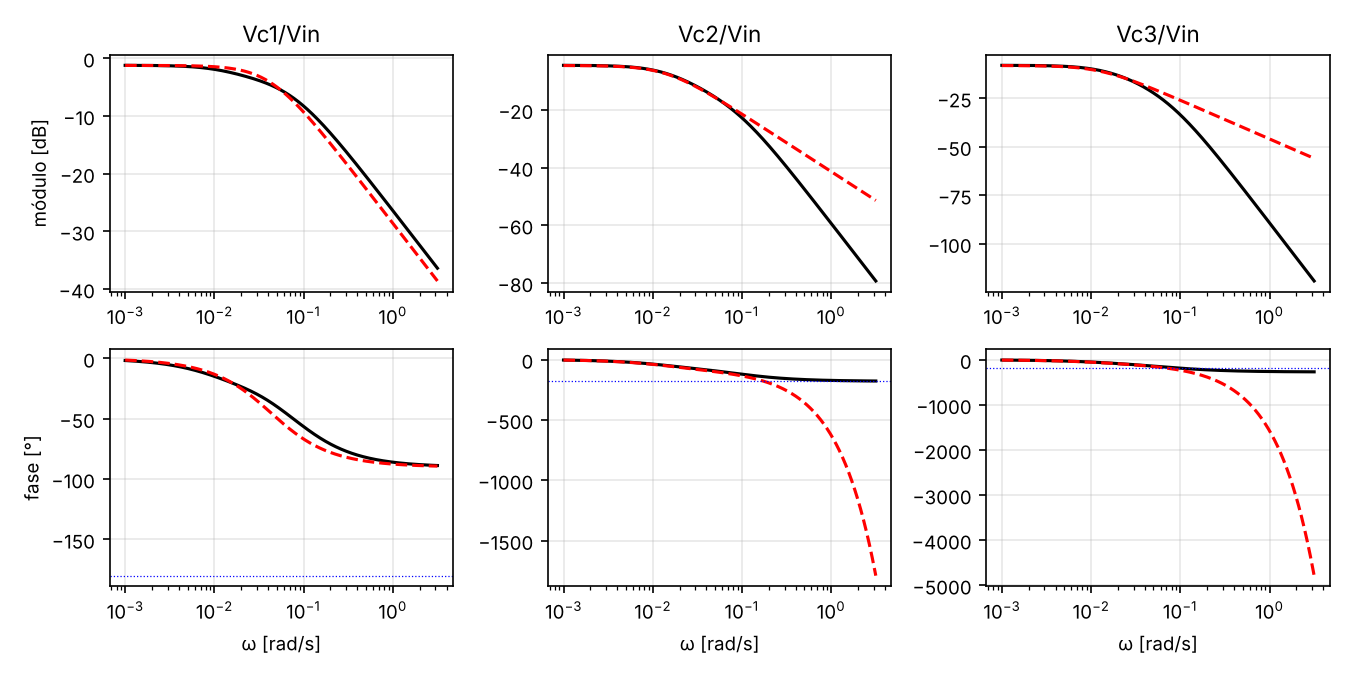
\includegraphics[width=.95\textwidth]{figs/bode.png}
\caption{Bode das FTs completas (preto) e reduzidas (vermelho tracejado).}\end{figure}
Valores em algumas frequências (módulo e fase em graus):
\begin{center}\small
\begin{tabular}{c|cc|cc|cc}\toprule
 & \multicolumn{2}{c|}{$\Vc1$ completa / reduzida} & \multicolumn{2}{c|}{$\Vc2$ completa} & \multicolumn{2}{c}{$\Vc3$ completa / reduzida}\\
$\omega$ [rad/s] & $|G|$ & $\angle G$ & $|G|$ & $\angle G$ & $|G|$ & $\angle G$ / red.\\\midrule
0,01 & 0,8016 (red 0,8445) & $-14{,}8$ ($-13{,}1$) & 0,4888 & $-37{,}7$ & 0,3215 & $-49{,}5$ ($-52{,}8$)\\
0,03 & 0,6503 (0,7106) & $-29{,}6$ ($-35{,}0$) & 0,2622 & $-74{,}9$ & 0,1492 & $-107{,}1$ ($-111{,}4$)\\
0,10 & 0,3854 (0,3419) & $-56{,}5$ ($-66{,}8$) & 0,0726 & $-121{,}3$ & 0,0210 & $-185{,}8$ ($-231{,}2$)\\
0,30 & 0,1550 (0,1228) & $-76{,}9$ ($-81{,}9$) & 0,0113 & $-156{,}7$ & 0,0012 & $-237{,}7$ ($-533{,}1$)\\\bottomrule
\end{tabular}\end{center}

\subsection{Margens de ganho e de fase}
Como $K<1$ em todas as plantas, o módulo da planta sozinha nunca chega a 0 dB: não existe cruzamento de ganho e a margem de fase seria infinita. Para obter margens com significado, fecho a malha com um controlador proporcional $K_c$ e comparo:
\begin{itemize}
\item o \textbf{ganho crítico} $K_{cu}=1/|G(j\omega_{180})|$, onde $\omega_{180}$ é a frequência em que a fase vale $-180^\circ$ (margem de ganho da planta);
\item a \textbf{margem de fase} $PM=180^\circ+\angle\big(K_cG(j\omega_g)\big)$, onde $|K_cG(j\omega_g)|=1$, para $K_c=3,5,10$.
\end{itemize}
\textbf{Cálculo exato de $K_{cu}$ para a FT completa de $\Vc3$ (critério de Routh).}
\begin{formula}Com $K_c$ puro, a equação característica é $1+K_cG(s)=0$. Para um polinômio $a_3s^3+a_2s^2+a_1s+a_0=0$, a linha $s^1$ da tabela de Routh é $\big[a_2a_1-a_3a_0\big]/a_2$; a estabilidade marginal ocorre quando essa linha se anula. O polinômio auxiliar é $a_2s^2+a_0=0$.\end{formula}
Aqui $a_3=11\,416{,}7$, $a_2=1978{,}65$, $a_1=95{,}071$, $a_0=1+K_cK_3$:
\[
a_2a_1=a_3(1+K_{cu}K_3)\ \Rightarrow\ 1+K_{cu}K_3=\frac{a_2a_1}{a_3}=\frac{1978{,}65\cdot95{,}071}{11\,416{,}7}=16{,}477
\]
\[
K_{cu}=\frac{16{,}477-1}{0{,}3971}=38{,}97 .
\]
Frequência de oscilação (polinômio auxiliar): $\omega_u^2=a_0/a_2=(1+K_{cu}K_3)/a_2=a_1/a_3$, logo
\[
\omega_u=\sqrt{\frac{95{,}071}{11\,416{,}7}}=\sqrt{0{,}008328}=0{,}09125\ \mathrm{rad/s},\qquad T_u=\frac{2\pi}{\omega_u}=\frac{6{,}2832}{0{,}09125}=68{,}85\ \mathrm{s}.
\]
\textbf{Para a FT reduzida de $\Vc3$.} Resolvo $-\arctan(\omega\tau)-\omega t_0=-\pi$, isto é, $f(\omega)=\pi-\arctan(78{,}03\omega)-25{,}92\omega=0$, por bisseção (em $f>0$ o ponto fica à esquerda da raiz):
\begin{center}\small
\begin{tabular}{cccc}\toprule passo & intervalo & ponto médio & $f$\\\midrule
1 & [0,010; 0,200] & 0,1050 & $-1{,}029$\\ 2 & [0,010; 0,1050] & 0,0575 & $+0{,}300$\\ 3 & [0,0575; 0,1050] & 0,0813 & $-0{,}379$\\ 4 & [0,0575; 0,0813] & 0,0694 & $-0{,}045$\\ 5 & [0,0575; 0,0694] & 0,0634 & $+0{,}126$\\ 6 & [0,0634; 0,0694] & 0,0664 & $+0{,}040$\\ $\vdots$ & & & \\\bottomrule
\end{tabular}\end{center}
Convergindo: $\omega_{180}=0{,}0678$ rad/s. Verificação: $\arctan(0{,}0678\cdot78{,}03=5{,}290)=79{,}3^\circ=1{,}384$ rad e $\omega t_0=0{,}0678\cdot25{,}92=1{,}757$ rad; soma $=3{,}141$ rad $=\pi$ $\checkmark$. Então
\[
K_{cu}=\frac{\sqrt{1+(\omega_{180}\tau)^2}}{K}=\frac{\sqrt{1+5{,}290^2}}{0{,}3918}=\frac{5{,}383}{0{,}3918}=13{,}74 .
\]
Para $\Vc2$ reduzida o mesmo procedimento dá $\omega_{180}=0{,}176$ rad/s e $K_{cu}=20{,}8$.

\textbf{$\Vc1$ e $\Vc2$ completas.} $\Vc1$ (3 polos, 2 zeros): a fase fica entre $0^\circ$ e $-90^\circ$, nunca chega a $-180^\circ$: $K_{cu}$ não existe. $\Vc2$ (3 polos, 1 zero): a fase tende a $-180^\circ$ por cima sem atingi-la (confirmado no gráfico e por Routh: a linha $s^1$ fica $a_2(a_1+K_cK_2\tau_z)-a_3(1+K_cK_2)>0$ para todo $K_c$, pois $a_2\tau_z>a_3$), também sem $K_{cu}$ finito.

\textbf{Margem de fase, exemplo completo ($\Vc3$ completa, $K_c=5$).} Procuro $\omega_g$ tal que $5|G(j\omega_g)|=1$, isto é, $|G|=0{,}2$. Por tentativa numérica: $\omega_g=0{,}0222$ rad/s. Fase nesse ponto:
\[
-\big[\arctan(0{,}0222\cdot68{,}68)+\arctan(0{,}0222\cdot16{,}00)+\arctan(0{,}0222\cdot10{,}39)\big]=-(56{,}7+19{,}5+13{,}0)=-89{,}3^\circ,
\]
\[
PM=180^\circ-89{,}3^\circ=90{,}7^\circ .
\]
\begin{center}
\begin{tabular}{lcccc}\toprule & & $\Vc1$ & $\Vc2$ & $\Vc3$\\\midrule
\multirow{2}{*}{$K_{cu}$ ($\omega_{180}$ [rad/s])} & completa & $\infty$ & $\infty$ & 39,0 (0,091)\\ & reduzida & $\infty$ & 20,8 (0,176) & 13,7 (0,068)\\\midrule
\multirow{2}{*}{$PM$, $K_c=3$} & completa & $118{,}7^\circ$ & $116{,}4^\circ$ & $134{,}9^\circ$\\ & reduzida & $112{,}6^\circ$ & $113{,}4^\circ$ & $136{,}5^\circ$\\\midrule
\multirow{2}{*}{$PM$, $K_c=5$} & completa & $107{,}0^\circ$ & $93{,}8^\circ$ & $90{,}7^\circ$\\ & reduzida & $103{,}3^\circ$ & $88{,}5^\circ$ & $88{,}6^\circ$\\\midrule
\multirow{2}{*}{$PM$, $K_c=10$} & completa & $98{,}4^\circ$ & $68{,}5^\circ$ & $52{,}1^\circ$\\ & reduzida & $96{,}6^\circ$ & $54{,}8^\circ$ & $32{,}7^\circ$\\\bottomrule
\end{tabular}\end{center}
\begin{just}\textbf{Margem de fase:} praticamente igual para $K_c=3$ e $5$ (diferenças de até $6^\circ$), porque o cruzamento de ganho ocorre em baixa frequência ($<0{,}05$ rad/s), onde a FOPDT reproduz bem a completa. Só com $K_c=10$ o prejuízo é visível ($\Vc3$: $52^\circ$ contra $33^\circ$). \textbf{Margem de ganho:} aqui há prejuízo, e é para o lado \emph{conservador}: o atraso $e^{-t_0s}$ da reduzida faz a fase cair sem limite, enquanto a completa satura em $-180^\circ$ ($\Vc2$) ou $-270^\circ$ ($\Vc3$). Assim a reduzida cruza $-180^\circ$ em frequência menor e prevê $K_{cu}=13{,}7$ contra $39{,}0$ ($\Vc3$): subestima a margem em $\sim$65\,\%. \textbf{Consequência:} sintonizar com a FOPDT é seguro (o ganho fica limitado pelo modelo reduzido), mas na planta real a malha tem mais folga do que a simulação reduzida indica. Já para o método de Ziegler--Nichols (item 4.1) o ganho crítico precisa ser o da planta completa, não o da reduzida.\end{just}

%==================== PARTE 2 ====================
\section{Método de simulação em malha fechada (comum aos itens)}
\subsection{Estrutura do PID (PI\_D paralelo do OpenPLC)}
\begin{formula}
$\displaystyle U(s)=\Big(K_p+\frac{K_i}{s}\Big)\big(R(s)-Y(s)\big)-D(s)\,Y(s),\qquad D(s)=\frac{K_d\,s}{\mu T_d\,s+1},\qquad K_i=\frac{K_p}{T_i},\ K_d=K_pT_d .$
\end{formula}
Aqui $R=SP$, $Y=VP$, $U=SC$ (sinal de controle). \begin{just}A ação proporcional e a integral atuam sobre o erro $e=SP-VP$; a derivada atua \emph{só sobre a VP} (e não sobre o erro) para não derivar os degraus do SP (``chute derivativo''). O filtro de constante $\mu T_d$ ($\mu=0{,}1$) limita o ganho do termo derivativo em alta frequência a $K_p(1+1/\mu)$ (a derivada pura amplificaria o ruído do ADC). É essa a implementação do OpenPLC citada no enunciado.\end{just}

\subsection{Funções de transferência de malha fechada}
Sendo $Y=GU$ e $PI(s)=K_p+K_i/s$:
\[
U=PI\,R-(PI+D)\,Y=PI\,R-(PI+D)\,G\,U\ \Rightarrow\ U\,[1+(PI+D)G]=PI\,R .
\]
\begin{res}
\[
\frac{U}{R}=\frac{PI}{1+(PI+D)G},\qquad \frac{Y}{R}=\frac{PI\,G}{1+(PI+D)G}.
\]
\end{res}
\textbf{Forma polinomial (para simular).} Escrevo $G=N_G/D_G$, $PI=(K_ps+K_i)/s$ e $D=K_ds/(\mu T_ds+1)$. Levando ao denominador comum $s(\mu T_ds+1)$:
\[\begin{gathered}
PI+D=\frac{(K_ps+K_i)(\mu T_ds+1)+K_ds^2}{s(\mu T_ds+1)}=\frac{C_n}{C_d},\\ C_n=(K_ps+K_i)(\mu T_ds+1)+K_ds^2,\ C_d=s(\mu T_ds+1).
\end{gathered}\]
Substituindo e simplificando (o fator $s$ de $C_d$ cancela com o $s$ do $PI$):
\[
\frac{Y}{R}=\frac{(K_ps+K_i)(\mu T_ds+1)\,N_G}{C_dD_G+C_nN_G},\qquad
\frac{U}{R}=\frac{(K_ps+K_i)(\mu T_ds+1)\,D_G}{C_dD_G+C_nN_G}.
\]
O denominador $C_dD_G+C_nN_G$ é o polinômio característico da malha fechada: seus polos dizem se a malha é estável. Simulo com a rotina \texttt{lsim} (a mesma do script do professor no MATLAB).

\subsection{Planta nas simulações e atraso por Padé}
Uso duas plantas $\Vc3/\Vin$: \textbf{(a) FT reduzida (FOPDT)} (eq.~\eqref{ft3} reduzida: $K=0{,}3918$, $\tau=78{,}03$, $t_0=25{,}92$) e \textbf{(b) FT completa}, eq.~\eqref{ft3}.
\begin{formula}Aproximação de Padé de ordem $n/n$ de $e^{-x}$: $\displaystyle e^{-x}\approx\frac{\sum_{k=0}^{n}(-1)^kc_kx^k}{\sum_{k=0}^{n}c_kx^k}$, $\ c_k=\frac{(2n-k)!\,n!}{(2n)!\,k!\,(n-k)!}$.\end{formula}
\begin{just}O atraso $e^{-t_0s}$ não é uma função racional, e \texttt{lsim} trabalha com polinômios. Com $t_0=25{,}92$ s, o Padé de 1ª ordem (usado no script do professor) distorce bastante; uso a de 3ª ordem ($n=3$).\end{just}
Para $n=3$: $c_0=1$; $c_1=\frac{5!\,3!}{6!\,1!\,2!}=\frac{720}{1440}=\frac12$; $c_2=\frac{4!\,3!}{6!\,2!\,1!}=\frac{144}{1440}=\frac1{10}$; $c_3=\frac{3!\,3!}{6!\,3!\,0!}=\frac{36}{4320}=\frac1{120}$. Com $x=t_0s$ e $t_0=25{,}92$:
\[
e^{-t_0s}\approx\frac{1-\frac{t_0s}{2}+\frac{(t_0s)^2}{10}-\frac{(t_0s)^3}{120}}{1+\frac{t_0s}{2}+\frac{(t_0s)^2}{10}+\frac{(t_0s)^3}{120}}
=\frac{-145{,}12\,s^3+67{,}18\,s^2-12{,}96\,s+1}{145{,}12\,s^3+67{,}18\,s^2+12{,}96\,s+1},
\]
pois $t_0/2=12{,}96$, $t_0^2/10=671{,}8/10=67{,}18$ e $t_0^3/120=17\,414/120=145{,}12$. Para garantir que o Padé não distorce, repeti o item 1.1 com o atraso exato (integração no tempo): diferença máxima na VP de 0,24\,\% da escala.

\subsection{Condições das simulações}
Partida em regime com $SP=SP_0$ e $SC=SP_0/K_{planta}$; em $t=50$ s o SP muda para $SP_1$. As simulações são \textbf{lineares}: não incluem a saturação do SC em 0--100\,\% e só valem enquanto o SC ficar entre esses limites (por isso escolho o degrau de SP de modo que o SC não sature). O valor máximo de $\Vc3$ em regime é $K_3\cdot100=39{,}7\,\%$.

\subsection{Conversão série $\to$ ideal (Eq.\ 5-3.17 do livro)}
\begin{formula}As Tabelas 7-1.1 e 7-4.1 dão o PID na forma real/série:
$\displaystyle C(s)=K_c'\Big(1+\frac1{\tau_I's}\Big)(1+\tau_D's)=K_c'\Big[1+\frac{\tau_D'}{\tau_I'}+\frac1{\tau_I's}+\tau_D's\Big]$,
e o PID ideal/paralelo é $C(s)=K_c\big[1+\frac1{\tau_Is}+\tau_Ds\big]$.\end{formula}
Igualando termo a termo:
\begin{itemize}
\item termo constante: $K_c=K_c'\Big(1+\dfrac{\tau_D'}{\tau_I'}\Big)$;
\item termo em $1/s$: $\dfrac{K_c}{\tau_I}=\dfrac{K_c'}{\tau_I'}\ \Rightarrow\ \tau_I=\tau_I'\,\dfrac{K_c}{K_c'}=\tau_I'\Big(1+\dfrac{\tau_D'}{\tau_I'}\Big)=\tau_I'+\tau_D'$;
\item termo em $s$: $K_c\tau_D=K_c'\tau_D'\ \Rightarrow\ \tau_D=\dfrac{K_c'\tau_D'}{K_c}=\dfrac{\tau_D'}{1+\tau_D'/\tau_I'}=\dfrac{\tau_I'\tau_D'}{\tau_I'+\tau_D'}$.
\end{itemize}
\begin{res}Para o OpenPLC: $K_p=K_c$, $K_i=K_c/\tau_I$, $K_d=K_c\tau_D$.\end{res}

%------------------------------------------------------------------
\section{Item 1.1: PID pela Tabela 7-4.1 (síntese direta)}
\subsection{O que é pedido}
``Uma sintonia de PID segundo o método da tabela 7-4.1 do livro, e verifique o sucesso da sintonia confrontando simulação com o experimental.'' Planta: $\Vc3/\Vin$, FOPDT com $K=0{,}3918$, $\tau=78{,}03$ s, $t_0=25{,}92$ s.

\subsection{De onde vem a tabela (dedução)}
\begin{formula}Síntese direta (Dahlin): escolho a resposta desejada de malha fechada $\dfrac YR=\dfrac{e^{-t_0s}}{\tau_cs+1}$ (1ª ordem com o mesmo atraso da planta) e calculo o controlador que a produz:
\[C(s)=\frac1{G(s)}\,\frac{Y/R}{1-Y/R}.\]\end{formula}
Com $G=\dfrac{Ke^{-t_0s}}{\tau s+1}$, tem-se $1/G=\dfrac{(\tau s+1)e^{t_0s}}{K}$ e
\[
\frac{Y/R}{1-Y/R}=\frac{e^{-t_0s}}{\tau_cs+1-e^{-t_0s}}\ \Rightarrow\ C(s)=\frac{\tau s+1}{K\,(\tau_cs+1-e^{-t_0s})}.
\]
Aproximando o atraso por Padé de 1ª ordem, $e^{-t_0s}\approx\dfrac{1-t_0s/2}{1+t_0s/2}$:
\[
\tau_cs+1-\frac{1-t_0s/2}{1+t_0s/2}=\frac{(\tau_cs+1)(1+\frac{t_0s}2)-(1-\frac{t_0s}2)}{1+\frac{t_0s}2}=\frac{s\big[(\tau_c+t_0)+\frac{\tau_ct_0}{2}s\big]}{1+\frac{t_0s}2},
\]
\[
C(s)=\frac{(\tau s+1)(1+\frac{t_0s}{2})}{K\,s\,\big[(\tau_c+t_0)+\frac{\tau_ct_0}{2}s\big]}
=\underbrace{\frac{\tau}{K(\tau_c+t_0)}}_{K_c'}\Big(1+\frac1{\tau s}\Big)\Big(1+\frac{t_0}{2}s\Big)\frac1{1+\tau_fs},\quad \tau_f=\frac{\tau_ct_0}{2(\tau_c+t_0)} .
\]
Desprezando o filtro $\tau_f$, obtém-se exatamente a linha de PID da Tabela 7-4.1 (forma real/série):
\[
K_c'=\frac{\tau}{K(t_0+\tau_c)},\qquad\tau_I'=\tau,\qquad\tau_D'=\frac{t_0}{2}.
\]
Convertendo para a forma ideal (Seção 7.5) obtém-se a fórmula do script do professor com $\lambda=\tau_c$:
\[
K_c=K_c'\Big(1+\frac{\tau_D'}{\tau_I'}\Big)=\frac{\tau}{K(t_0+\tau_c)}\cdot\frac{2\tau+t_0}{2\tau}=\frac{2\tau+t_0}{2K(\tau_c+t_0)},\quad T_i=\tau+\frac{t_0}2,\quad T_d=\frac{\tau\,t_0/2}{\tau+t_0/2}=\frac{\tau t_0}{2\tau+t_0}.
\]
O único parâmetro de projeto é $\tau_c$ (constante de tempo desejada de malha fechada).

\subsection{Escolha de $\tau_c$}
Testei $\tau_c=20,30,40$ e $60$ s com degrau de SP de 20 para 30\,\% (alcançável, pois o máximo é 39,7\,\%). Resultados (FOPDT / FT completa):
\begin{center}\small
\begin{tabular}{rcccccc}\toprule $\tau_c$ [s] & $K_p$ & $K_i$ & $K_d$ & sobress.\ [\%] & $t_{63,2}$ [s] & pico do SC [\%]\\\midrule
20 & 5,057 & 0,0556 & 56,21 & 2,7 / 2,4 & 51,5 / 54,4 & 114 / 103\\
30 & 4,153 & 0,0456 & 46,16 & 1,5 / 0,6 & 59,0 / 62,0 & 102 / 94\\
\textbf{40} & \textbf{3,523} & \textbf{0,0387} & \textbf{39,15} & 0,7 / 0,0 & 67,9 / 69,6 & 94 / 88\\
60 & 2,703 & 0,0297 & 30,04 & 0,1 / 0,0 & 86,9 / 85,3 & 84 / 80\\\bottomrule
\end{tabular}\end{center}
Em todos os casos $T_i=90{,}99$ s e $T_d=11{,}11$ s (não dependem de $\tau_c$).
\begin{figure}[H]\centering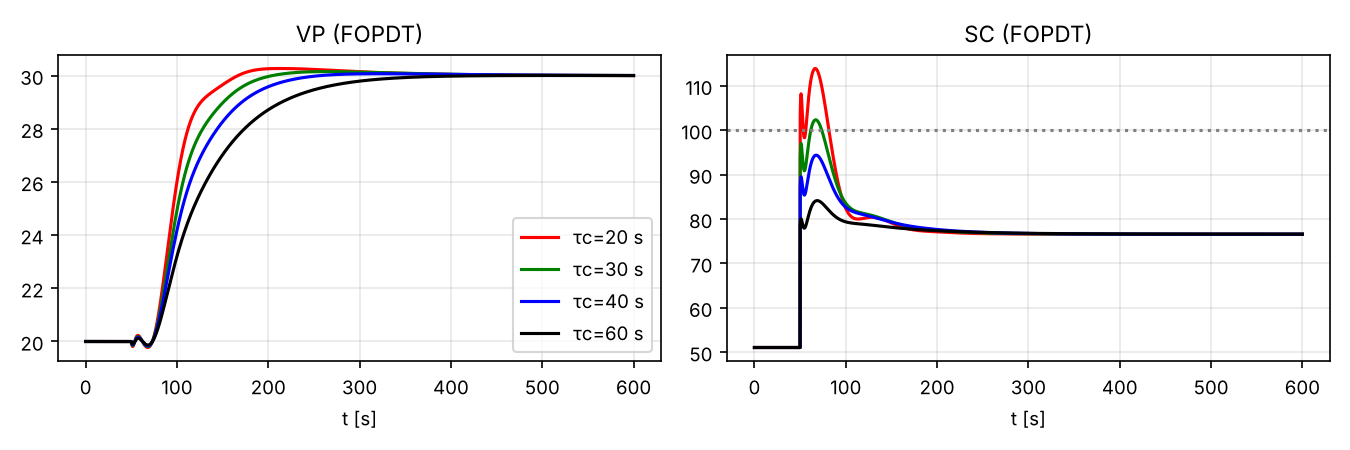
\includegraphics[width=.95\textwidth]{figs/i11_tc.png}\caption{Efeito de $\tau_c$ na VP e no SC (simulação com FOPDT).}\end{figure}
\begin{just}Adoto $\tau_c=40$ s. Com 20 e 30 s o SC da simulação passa de 100\,\% (na bancada o SC saturaria e a simulação linear deixaria de valer). Com 60 s a resposta fica lenta (63,2\,\% em 87 s) sem ganho real. Com 40 s o pico do SC é 94\,\% e o sobressinal é menor que 1\,\%. Além disso $\tau_c=40$ s é maior que o atraso $t_0=25{,}9$ s, o que mantém a malha robusta ao tempo morto. O script do professor usa $\lambda=60$ s (para a planta dele, $\tau=82{,}5$ s); se ele indicar outro valor, basta trocar $\tau_c$ nas fórmulas.\end{just}

\subsection{Cálculo passo a passo ($\tau_c=40$ s)}
\textbf{Passo 1 --- forma real/série (Tabela 7-4.1):}
\[
K_c'=\frac{\tau}{K(t_0+\tau_c)}=\frac{78{,}03}{0{,}3918\,(25{,}92+40)}=\frac{78{,}03}{0{,}3918\cdot65{,}92}=\frac{78{,}03}{25{,}83}=3{,}021\ \%\mathrm{SC}/\%\mathrm{VP},
\]
\[
\tau_I'=\tau=78{,}03\ \mathrm{s},\qquad \tau_D'=\frac{t_0}2=\frac{25{,}92}{2}=12{,}96\ \mathrm{s}.
\]
\textbf{Passo 2 --- conversão para a forma ideal (Seção 7.5):}
\[
K_p=K_c'\Big(1+\frac{\tau_D'}{\tau_I'}\Big)=3{,}021\Big(1+\frac{12{,}96}{78{,}03}\Big)=3{,}021\cdot1{,}1661=3{,}523,
\]
\[
T_i=\tau_I'+\tau_D'=78{,}03+12{,}96=90{,}99\ \mathrm{s},\qquad T_d=\frac{\tau_I'\tau_D'}{\tau_I'+\tau_D'}=\frac{78{,}03\cdot12{,}96}{90{,}99}=\frac{1011{,}2}{90{,}99}=11{,}11\ \mathrm{s}.
\]
\textbf{Conferência com a fórmula direta (script do professor):} $K_p=\dfrac{2\cdot78{,}03+25{,}92}{2\cdot0{,}3918\cdot(40+25{,}92)}=\dfrac{181{,}98}{51{,}66}=3{,}523$ $\checkmark$.

\textbf{Passo 3 --- parâmetros do PI\_D paralelo do OpenPLC:}
\[\begin{gathered}
K_i=\frac{K_p}{T_i}=\frac{3{,}523}{90{,}99}=0{,}03872\ \mathrm{s^{-1}},\\ K_d=K_pT_d=3{,}523\cdot11{,}11=39{,}15\ \mathrm{s},\\ \mu T_d=0{,}1\cdot11{,}11=1{,}11\ \mathrm{s}.
\end{gathered}\]
\begin{res}$K_p=3{,}523$;\quad $K_i=0{,}03872$ (ou $T_i=90{,}99$ s);\quad $K_d=39{,}15$ (ou $T_d=11{,}11$ s);\quad $\mu=0{,}1$.\\
Lei de controle: $SC(t)=K_pe(t)+K_i\!\int e\,dt-K_d\dfrac{d}{dt}VP_{filtrada}(t)$.\end{res}

\subsection{Simulação}
Degrau de SP de 20 para 30\,\% em $t=50$ s, partindo do regime com $SC_0=20/K\approx51{,}0\,\%$ (FOPDT) e $50{,}4\,\%$ (FT completa, $K_3=0{,}3971$). \emph{Comportamento imediato do SC:} em $t=50$ s o termo proporcional dá um salto $K_p\Delta SP=3{,}523\cdot10=35{,}2$ pontos (de 51,0 para $\approx86$\,\%); a derivada não contribui com ``chute'' porque age só sobre a VP.
\begin{figure}[H]\centering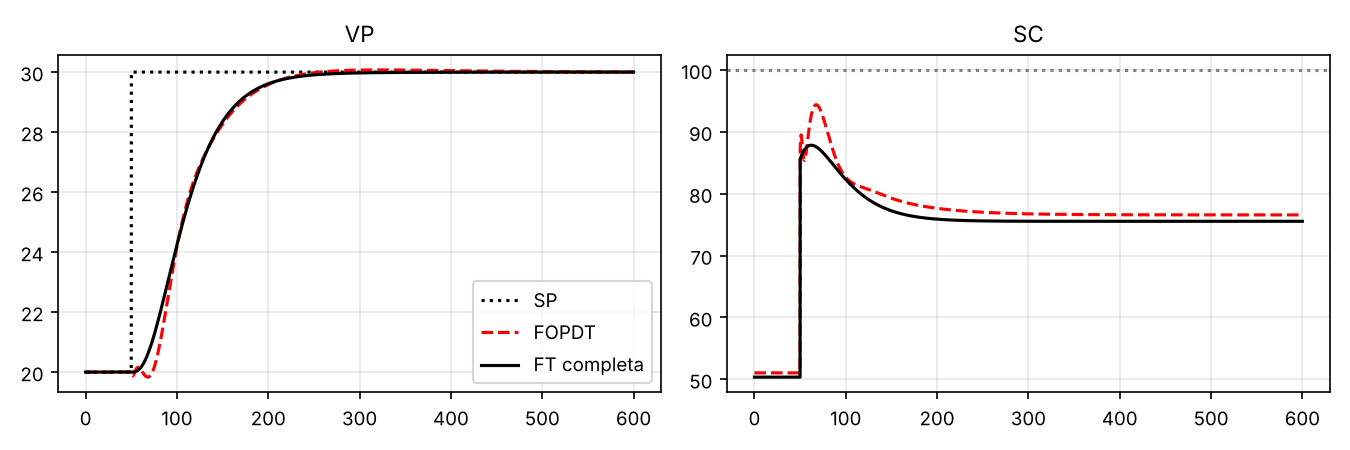
\includegraphics[width=.95\textwidth]{figs/i11.png}\caption{Item 1.1: VP e SC simulados (FOPDT em vermelho tracejado; FT completa em preto).}\end{figure}
\begin{center}\small
\begin{tabular}{lccccc}\toprule & sobress.\ [\%] & $t_{63,2}$ [s] & $t_s$ ($\pm2\%$) [s] & pico do SC [\%] & SC final [\%]\\\midrule
FOPDT & 0,7 & 67,9 & 169,6 & 94,4 & 76,6\\ FT completa & 0,0 & 69,6 & 172,8 & 87,8 & 75,5\\\bottomrule\end{tabular}\end{center}
$SC_{final}=SP_1/K$: $30/0{,}3918=76{,}6$ (FOPDT) e $30/0{,}3971=75{,}5$ (completa); a diferença vem de $K$ ($1{,}3\,\%$).

\textbf{Polos de malha fechada} (raízes de $C_dD_G+C_nN_G$, com Padé de 3ª ordem): FOPDT: $-0{,}511\pm0{,}397j$, $-0{,}0638\pm0{,}0903j$, $-0{,}0182$, $-0{,}0130$; FT completa: $-0{,}902$, $-0{,}0832$, $-0{,}0422$, $-0{,}0351$, $-0{,}0109$. Todos com parte real negativa $\Rightarrow$ malha estável nos dois modelos.

\textbf{Margens da malha aberta $L=(PI+D)G$:} FOPDT: $GM=3{,}7$ (11,4 dB), $PM=78{,}4^\circ$; FT completa: $GM=59{,}7$ (35,5 dB), $PM=81{,}4^\circ$. A margem de fase é praticamente igual nos dois modelos; a margem de ganho da FOPDT é muito menor, como visto na Seção 6.2.
\begin{just}Os dois modelos concordam no formato e na escala de tempo da VP. A FOPDT mostra um pequeno sobressinal e um pico de SC maior (94 contra 88\,\%) porque seu atraso puro e o ganho um pouco diferente alteram a ação proporcional+derivativa.\end{just}
\begin{todo}Procedimento: (i) medir $R$ e $C$ e conferir $K$, $\tau$, $t_0$ pelo degrau em malha aberta; (ii) malha aberta com SO$=20/K\approx50{,}4\,\%$ até $\Vc3\approx20\,\%$; (iii) passar a automático com $SP=VP$ e os parâmetros acima (conferir se o bloco pede $K_p$, $K_i$, $K_d$ ou $K_p$, $T_i$, $T_d$); (iv) aplicar $SP$: 20 $\to$ 30\,\% e gravar SO, SP, VP. Confrontar VP exp.\ $\times$ simulada e SC exp.\ ($=$ SO) $\times$ simulado (figura acima). Resultados: \underline{\hspace{6cm}}\end{todo}

%------------------------------------------------------------------
\section{Item 2.1: PID 2GL (método do $\alpha$ de Juliana Dalmaso)}
\subsection{O que é pedido}
``Uma sintonia do PID 2GL seguindo a mesma metodologia adotada no TCC de Juliana Dalmaso da Silva para escolha do alfa e verifique o sucesso da sintonia confrontando simulação com o experimental quando é aplicado um degrau no SP.''

\subsection{A metodologia do TCC}
Com PID de 1 grau de liberdade, a malha fechada é $VP=\dfrac{PID\,H}{1+PID\,H}SP+\dfrac{H}{1+PID\,H}D$ ($H$ = planta, $D$ = distúrbio). Uma única sintonia não otimiza as duas respostas: a sintonia \emph{servo} (boa para SP) tem ganho menor e a \emph{regulatória} (boa para distúrbio) tem ganho maior, mas ao mudar o SP exige muito do atuador e satura o SC. O PID 2GL resolve isso colocando um filtro no SP:
\begin{formula}
$\displaystyle C_f(s)=\frac{(1-\alpha)T_is+1}{T_is+1},\qquad VP=\frac{C_f\,PI\,G}{1+(PI+D)G}\,SP+\frac{G}{1+(PI+D)G}\,D .$
\end{formula}
\begin{just}$C_f$ aparece \emph{só} na resposta ao SP; a resposta ao distúrbio fica a da sintonia regulatória, qualquer que seja $\alpha$. O filtro é um avanço--atraso. Para ver o efeito, multiplique $C_f$ pelo $PI=K_p\dfrac{T_is+1}{T_is}$: o zero $(T_is+1)$ do PI cancela o polo de $C_f$ e fica $C_f\,PI=K_p\dfrac{(1-\alpha)T_is+1}{T_is}$. Com $\alpha=0$ é o PI\_D comum; com $\alpha\to1$ vira $K_p/(T_is)$, isto é, o SP entra só pela integral (resposta suave, sem salto proporcional no SC).\end{just}
O TCC tem quatro passos: (1) sintonizar o PID para \textbf{controle regulatório} (síntese direta com $\tau_c$ pequeno); (2) sintonizar um PID para \textbf{controle servo} (mesma síntese com $\tau_c$ grande, no TCC $\tau_c=\tau$) e simulá-lo só como \emph{referência} da resposta desejada ao SP; (3) simular o 2GL variando $\alpha$ (no TCC: 0,4; 0,7; 0,99); (4) escolher o $\alpha$ cuja resposta ao SP fica mais próxima da servo, observando que o SC fique menor que o do regulatório (no TCC o $\alpha=0{,}7$ foi o escolhido).

\subsection{Passos 1 e 2: sintonias regulatória e servo}
Mesma fórmula do item 1.1, mudando $\tau_c$. Servo: $\tau_c=\tau=78{,}03$ s. Regulatório: $\tau_c=20$ s (pequeno, mas não menor que o razoável para $t_0=25{,}9$ s; com FOPDT: $GM=2{,}6$, $PM=73^\circ$).
\begin{align*}
\text{servo:}\ K_c'&=\frac{78{,}03}{0{,}3918\,(25{,}92+78{,}03)}=\frac{78{,}03}{0{,}3918\cdot103{,}95}=\frac{78{,}03}{40{,}73}=1{,}916\\ &\Rightarrow K_p=1{,}916\cdot1{,}1661=2{,}234\\
\text{regulatório:}\ K_c'&=\frac{78{,}03}{0{,}3918\,(25{,}92+20)}=\frac{78{,}03}{0{,}3918\cdot45{,}92}=\frac{78{,}03}{17{,}99}=4{,}337\\ &\Rightarrow K_p=4{,}337\cdot1{,}1661=5{,}057
\end{align*}
Nos dois casos $T_i=90{,}99$ s e $T_d=11{,}11$ s (não dependem de $\tau_c$). Regulatório: $K_i=5{,}057/90{,}99=0{,}05558$, $K_d=5{,}057\cdot11{,}11=56{,}21$. Servo: $K_i=2{,}234/90{,}99=0{,}02455$, $K_d=2{,}234\cdot11{,}11=24{,}83$. Como esperado pelo TCC, \textbf{o ganho do regulatório ($K_p=5{,}06$) é maior que o do servo ($2{,}23$).}

\subsection{Passos 3 e 4: escolha do $\alpha$}
Simulei o 2GL (regulatório + $C_f$) com $\alpha=0{,}4$; $0{,}7$; $0{,}99$ (valores do TCC) e fiz também uma varredura de $\alpha$ de 0 a 0,99 em passos de 0,01, medindo o erro RMS entre a VP do 2GL e a VP servo (referência) em $50<t<550$ s, em \% do degrau:
\[
\varepsilon(\alpha)=\frac{100}{\Delta SP}\sqrt{\frac1N\sum_k\big(VP_{2GL}(t_k;\alpha)-VP_{servo}(t_k)\big)^2},\qquad \Delta SP=10\,\%.
\]
\begin{figure}[H]\centering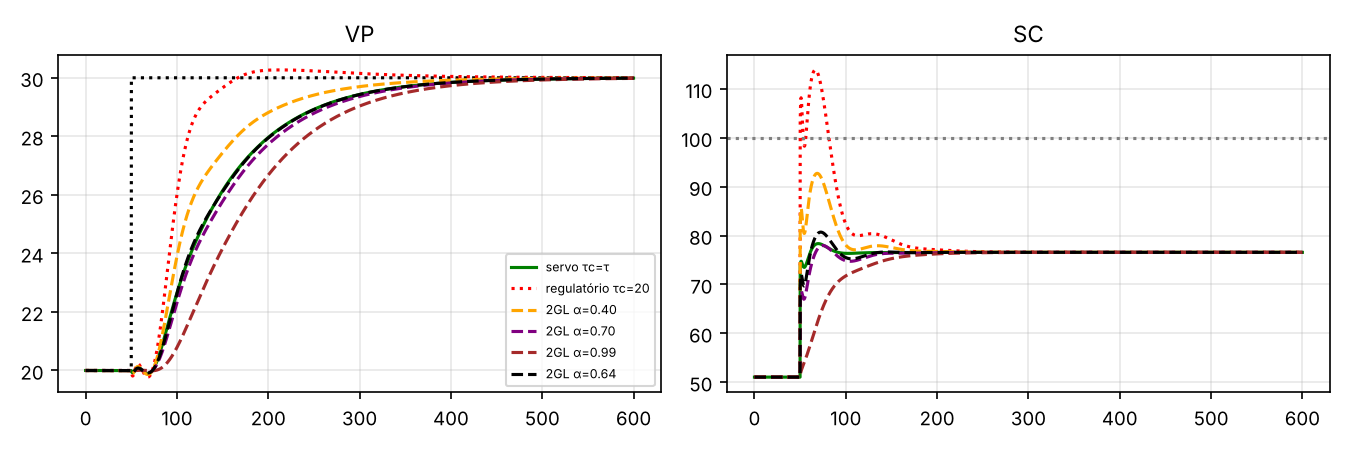
\includegraphics[width=.95\textwidth]{figs/i21.png}\caption{Item 2.1: PI\_D servo (verde), regulatório (vermelho pontilhado) e 2GL para $\alpha=0{,}4$; $0{,}7$; $0{,}99$ e $0{,}64$ (preto). Simulação com FOPDT.}\end{figure}
\begin{figure}[H]\centering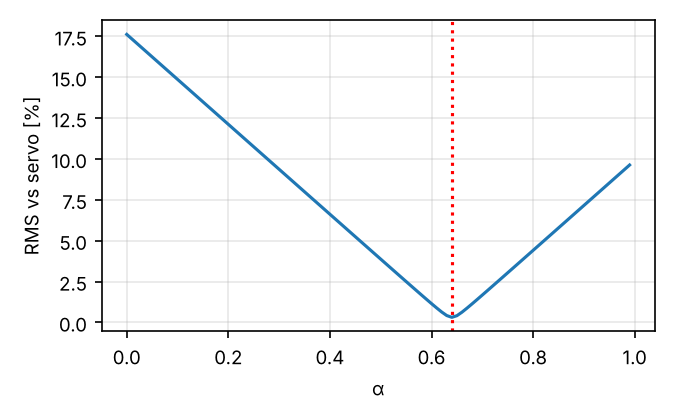
\includegraphics[width=.5\textwidth]{figs/i21_alpha.png}\caption{Erro RMS entre a VP do 2GL e a VP servo em função de $\alpha$.}\end{figure}
\begin{center}\small
\begin{tabular}{lcccc}\toprule Caso (FOPDT) & sobress.\ [\%] & $t_{63,2}$ [s] & pico do SC [\%] & RMS $\times$ servo [\%]\\\midrule
PI\_D servo ($\tau_c=\tau$) & 0,0 & 104 & 78 & (referência)\\
PI\_D regulatório ($\tau_c=20$) & 2,7 & 51,5 & 114 & 17,6\\
2GL $\alpha=0{,}40$ & 0,0 & 74,4 & 92,7 & 6,62\\
2GL $\alpha=0{,}70$ & 0,0 & 111,4 & 78,0 & 1,67\\
2GL $\alpha=0{,}99$ & 0,0 & 141,3 & 76,6 & 9,63\\
\textbf{2GL $\alpha=0{,}64$} & 0,0 & 104,5 & 80,7 & \textbf{0,31}\\\bottomrule\end{tabular}\end{center}
O mínimo ocorre em $\alpha=0{,}64$ com $\varepsilon=0{,}31\,\%$.
\begin{just}$\alpha=0{,}4$ ainda é rápido demais (RMS 6,6\,\%) e o SC chega a 93\,\%; $\alpha=0{,}99$ é lento demais (RMS 9,6\,\%, $t_{63}=141$ s). O valor $\alpha=0{,}7$ do TCC dá RMS 1,7\,\% e funciona, mas a varredura mostra que $\alpha=0{,}64$ reproduz ainda melhor a resposta servo (RMS 0,31\,\%), porque o $\alpha$ ótimo depende da planta (aqui, FOPDT com atraso; no TCC era um processo de 1ª ordem sem atraso). Adoto $\alpha=0{,}64$, mantendo a mesma metodologia do TCC (escolha por simulação do $\alpha$ que aproxima o servo, com SC menor que o do regulatório: pico de 81\,\% contra 114\,\%, que satura).\end{just}
Com a FT completa: $t_{63}=102{,}6$ s e pico do SC de 75,5\,\%.

\subsection{Parâmetros finais para o OpenPLC (PI\_D2GL)}
\begin{res}$K_p=5{,}057$;\quad $K_i=0{,}05558\ \mathrm{s^{-1}}$ ($T_i=90{,}99$ s);\quad $K_d=56{,}21$ ($T_d=11{,}11$ s);\quad $\mu=0{,}1$;\quad $\alpha=0{,}64$ (filtro do SP com $\beta=1$ fixo, como no CLP Omron do TCC).\end{res}
\begin{todo}Passar a automático com $SP=VP$ e os parâmetros acima; aplicar degrau de SP 20 $\to$ 30\,\%; gravar SO, SP, VP. Confrontar VP e SC com a simulação (FOPDT e FT completa). Se possível repetir com $\alpha=0$ (PI\_D regulatório comum) para mostrar o efeito de $\alpha$ (SC chegando a 114\,\%, isto é, saturando). Resultados: \underline{\hspace{6cm}}\end{todo}

%------------------------------------------------------------------
\section{Item 3.1: integral do erro mínimo (seção 7-2.3)}
\subsection{O método}
Na seção 7-2.3 o livro apresenta correlações que minimizam um índice de integral do erro, aqui $\mathrm{IAE}=\int_0^\infty|e|\,dt$, para plantas FOPDT. Para o PID ideal, com $r=t_0/\tau$ (válido para $0{,}1<r<1$):
\begin{formula}
\textbf{Tabela 7-2.3 (ponto fixo, Rovira):}\quad $K_c=\dfrac{1{,}086}{K}\,r^{-0{,}869},\quad \tau_I=\dfrac{\tau}{0{,}740-0{,}130\,r},\quad \tau_D=0{,}348\,\tau\,r^{0{,}914}$.\\[3pt]
\textbf{Tabela 7-2.2 (distúrbio, López):}\quad $K_c=\dfrac{1{,}435}{K}\,r^{-0{,}921},\quad \tau_I=\dfrac{\tau}{0{,}878}\,r^{0{,}749},\quad \tau_D=0{,}482\,\tau\,r^{1{,}137}$.
\end{formula}
\begin{just}Como o experimento é um degrau no SP (como nos outros itens), a sintonia principal é a da Tabela 7-2.3 (ponto fixo); calculo também a de distúrbio para comparar. Aqui $r=25{,}92/78{,}03=0{,}3322$, dentro da faixa de validade. As tabelas já fornecem o PID na forma ideal (paralela), então \textbf{não há conversão série$\to$ideal}: $K_p=K_c$, $K_i=K_c/\tau_I$, $K_d=K_c\tau_D$.\end{just}

\subsection{Cálculo passo a passo}
Potências calculadas por logaritmo: $\ln r=\ln0{,}3322=-1{,}1021$.

\textbf{Ponto fixo (Tabela 7-2.3):}
\begin{align*}
r^{-0{,}869}&=e^{-0{,}869\cdot(-1{,}1021)}=e^{0{,}9577}=2{,}606\\
\frac{1{,}086}{K}&=\frac{1{,}086}{0{,}3918}=2{,}772\\
K_p&=2{,}772\cdot2{,}606=\mathbf{7{,}222}\\
T_i&=\frac{78{,}03}{0{,}740-0{,}130\cdot0{,}3322}=\frac{78{,}03}{0{,}740-0{,}0432}=\frac{78{,}03}{0{,}6968}=\mathbf{111{,}98\ s}\\
r^{0{,}914}&=e^{0{,}914\cdot(-1{,}1021)}=e^{-1{,}0073}=0{,}3652\\T_d&=0{,}348\cdot78{,}03\cdot0{,}3652=27{,}15\cdot0{,}3652=\mathbf{9{,}92\ s}\\
K_i&=\frac{K_p}{T_i}=\frac{7{,}222}{111{,}98}=\mathbf{0{,}06449}\\K_d&=K_pT_d=7{,}222\cdot9{,}917=\mathbf{71{,}63}
\end{align*}
\textbf{Distúrbio (Tabela 7-2.2), para comparar:}
\begin{align*}
r^{-0{,}921}&=e^{1{,}0150}=2{,}759\\K_p&=\frac{1{,}435}{0{,}3918}\cdot2{,}759=3{,}663\cdot2{,}759=10{,}11\\
r^{0{,}749}&=e^{-0{,}8254}=0{,}4380\\T_i&=\frac{78{,}03}{0{,}878}\cdot0{,}4380=38{,}93\ \mathrm{s}\\
r^{1{,}137}&=e^{-1{,}2531}=0{,}2856\\T_d&=0{,}482\cdot78{,}03\cdot0{,}2856=10{,}74\ \mathrm{s}\\
K_i&=10{,}11/38{,}93=0{,}2596\\K_d&=10{,}11\cdot10{,}74=108{,}6
\end{align*}
\begin{res}Ponto fixo: $K_p=7{,}222$; $K_i=0{,}06449$ ($T_i=111{,}98$ s); $K_d=71{,}63$ ($T_d=9{,}92$ s); $\mu=0{,}1$.\end{res}

\subsection{Simulação}
Degrau de SP de 20 para 25\,\% em $t=50$ s (menor que nos outros itens porque o ganho alto desta sintonia faria o SC passar de 100\,\% com 20 $\to$ 30\,\%).
\begin{figure}[H]\centering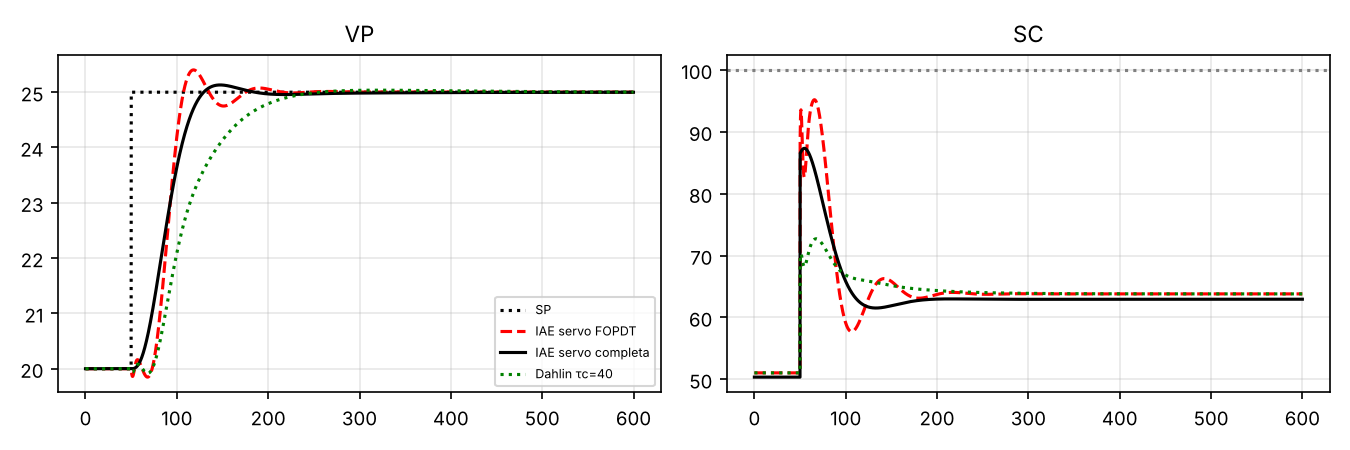
\includegraphics[width=.95\textwidth]{figs/i31.png}\caption{Item 3.1: IAE ponto fixo (FOPDT tracejado vermelho; FT completa preto) e Dahlin $\tau_c=40$ s do item 1.1 (verde pontilhado), degrau 20 $\to$ 25\,\%.}\end{figure}
\begin{center}\small
\begin{tabular}{lcccc}\toprule Sintonia (20 $\to$ 25\,\%), FOPDT / completa & sobress.\ [\%] & $t_{63,2}$ [s] & $t_s$ [s] & pico do SC [\%]\\\midrule
IAE ponto fixo (7-2.3) & 8,1 / 2,6 & 43,7 / 44,4 & 117 / 110 & 95 / 87\\
IAE distúrbio (7-2.2) & 83,6 / 42,3 & 37,8 / 33,3 & 227 / 201 & 129 / 107\\
Dahlin $\tau_c=40$ s (item 1.1) & 0,7 / 0,0 & 67,9 / 69,6 & 170 / 173 & 73 / 69\\\bottomrule\end{tabular}\end{center}
Margens da malha aberta com a sintonia de ponto fixo: FOPDT $GM=1{,}9$, $PM=64^\circ$; FT completa $GM=32{,}0$, $PM=71^\circ$.
\begin{just}A sintonia de ponto fixo é a mais rápida ($t_{63}=44$ s contra 68 s do Dahlin), à custa de sobressinal maior (8,1\,\% na FOPDT, 2,6\,\% na completa) e de $K_p$ mais alto --- esperado de um método que minimiza o erro integral sem penalizar o esforço de controle. A sintonia de distúrbio é ainda mais agressiva e, aplicada a um degrau de SP, produz sobressinal de 84\,\% na FOPDT: foi projetada para rejeitar distúrbios, não para seguir SP (a ideia do TCC: servo e regulatório exigem sintonias diferentes). A diferença de sobressinal entre FOPDT e completa vem do atraso puro da FOPDT, que reduz a margem de ganho (1,9 contra 32).\end{just}
\begin{todo}Mesmo procedimento do item 1.1 com $K_p=7{,}222$, $K_i=0{,}06449$, $K_d=71{,}63$, $\mu=0{,}1$ e degrau de SP 20 $\to$ 25\,\%. Confrontar VP e SC com a figura. Resultados: \underline{\hspace{6cm}}\end{todo}

%------------------------------------------------------------------
\section{Item 4.1: Ziegler--Nichols de razão de decaimento 1/4 (Tabela 7-1.1)}
\subsection{O método}
A Tabela 7-1.1 usa o \textbf{ganho final} $K_{cu}$ e o \textbf{período final} $T_u$: com controle só proporcional, aumenta-se $K_c$ até a VP oscilar com amplitude constante; $K_{cu}$ é esse ganho e $T_u$ o período da oscilação. Para o PID (forma real/série), razão de decaimento 1/4 (cada pico é 1/4 do anterior):
\begin{formula}$K_c'=\dfrac{K_{cu}}{1{,}7},\qquad\tau_I'=\dfrac{T_u}{2},\qquad\tau_D'=\dfrac{T_u}{8}$, convertidos à forma ideal pela Seção 7.5.\end{formula}
\subsection{$K_{cu}$ e $T_u$}
Experimentalmente serão medidos na bancada (teste de ganho final). Para poder simular, calculo-os da FT completa de $\Vc3$ pelo critério de Routh (Seção 6.2): $K_{cu}=38{,}97$, $\omega_u=0{,}09125$ rad/s, $T_u=68{,}85$ s. Confirmação pelos polos de $1+K_cG(s)=0$:
\begin{center}\small\begin{tabular}{ccc}\toprule $K_c$ & polos complexos dominantes & comportamento\\\midrule
$0{,}5K_{cu}=19{,}5$ & $-0{,}0108\pm0{,}0702j$ & oscilação amortece\\
$K_{cu}=39{,}0$ & $\approx0\pm0{,}0913j$ & oscilação sustentada, $T_u=2\pi/0{,}0913=68{,}85$ s\\
$1{,}2K_{cu}=46{,}8$ & $+0{,}0033\pm0{,}0975j$ & oscilação cresce (instável)\\\bottomrule\end{tabular}\end{center}
\begin{figure}[H]\centering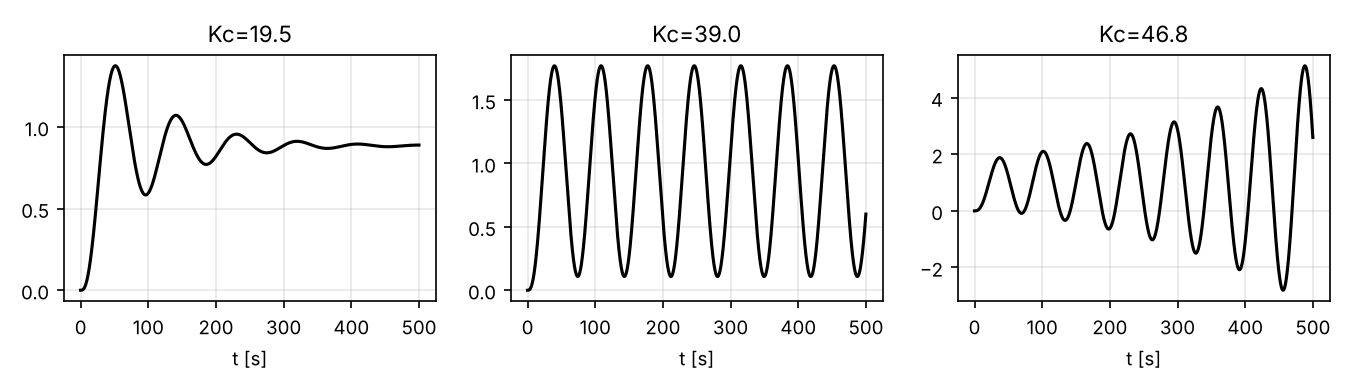
\includegraphics[width=.95\textwidth]{figs/i41_kcu.png}\caption{Teste de ganho final simulado (FT completa, $K_c$ puro, degrau no SP).}\end{figure}
\begin{just}Uso a FT \emph{completa} (e não a reduzida) para obter $K_{cu}$ e $T_u$ porque o método de Ziegler--Nichols exige o comportamento real da planta no limite de estabilidade. A FOPDT daria $K_{cu}=13{,}7$ e $T_u=92{,}7$ s, bem diferentes do real (39,0 e 68,9 s). Na bancada a oscilação sustentada será limitada pela saturação do SC em 0--100\,\%; deve-se registrar o menor $K_c$ que sustenta a oscilação e o período $T_u$ medido, e recalcular os parâmetros com as mesmas fórmulas abaixo.\end{just}

\subsection{Cálculo passo a passo}
\textbf{Passo 1 --- forma real/série:}
\[
K_c'=\frac{K_{cu}}{1{,}7}=\frac{38{,}97}{1{,}7}=22{,}92,\qquad\tau_I'=\frac{T_u}2=\frac{68{,}85}{2}=34{,}43\ \mathrm{s},\qquad\tau_D'=\frac{T_u}8=\frac{68{,}85}{8}=8{,}607\ \mathrm{s}.
\]
\textbf{Passo 2 --- forma ideal (Seção 7.5):}
\[
K_p=K_c'\Big(1+\frac{\tau_D'}{\tau_I'}\Big)=22{,}92\Big(1+\frac{8{,}607}{34{,}43}\Big)=22{,}92\cdot1{,}25=28{,}65,
\]
\[
T_i=\tau_I'+\tau_D'=34{,}43+8{,}607=43{,}03\ \mathrm{s},\qquad T_d=\frac{34{,}43\cdot8{,}607}{43{,}03}=\frac{296{,}3}{43{,}03}=6{,}885\ \mathrm{s}.
\]
\emph{Conferência por fórmula direta:} como $\tau_D'/\tau_I'=1/4$ sempre, $K_p=1{,}25\,K_{cu}/1{,}7=0{,}735K_{cu}=28{,}65$, $T_i=\frac58T_u=43{,}03$ s e $T_d=\frac1{10}T_u=6{,}885$ s $\checkmark$.

\textbf{Passo 3 --- OpenPLC:}
\[
K_i=\frac{K_p}{T_i}=\frac{28{,}65}{43{,}03}=0{,}6659\ \mathrm{s^{-1}},\qquad K_d=K_pT_d=28{,}65\cdot6{,}885=197{,}3\ \mathrm{s},\qquad\mu=0{,}1 .
\]
O ganho em alta frequência do PID (com o filtro $\mu=0{,}1$) é $K_p(1+1/\mu)=28{,}65\cdot11\approx315$: controlador de ganho alto, sensível a ruído de medição (a quantização do ADC é 0,098\,\%).
\begin{res}$K_p=28{,}65$;\ $K_i=0{,}6659$ ($T_i=43{,}03$ s);\ $K_d=197{,}3$ ($T_d=6{,}885$ s);\ $\mu=0{,}1$.\end{res}

\subsection{Simulação}
Degrau de SP de 10 para 12\,\% em $t=50$ s (pequeno porque o ganho alto faria o SC saturar em degraus maiores); $SC_0=10/0{,}3971=25{,}2\,\%$.
\begin{figure}[H]\centering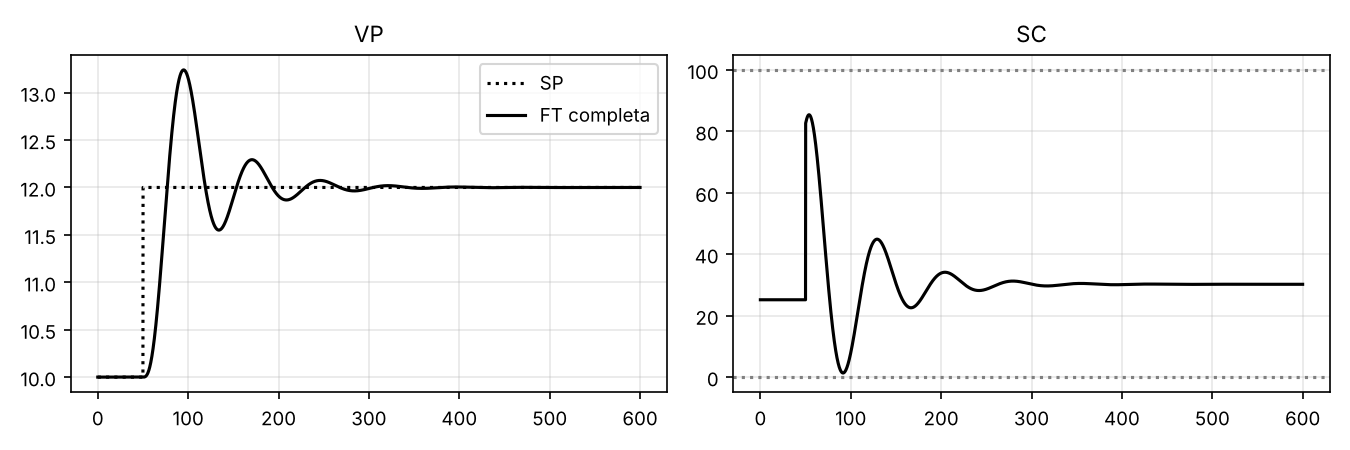
\includegraphics[width=.95\textwidth]{figs/i41.png}\caption{Item 4.1: PID de Ziegler--Nichols simulado com a FT completa.}\end{figure}
\begin{center}\small\begin{tabular}{lccccc}\toprule & sobress.\ [\%] & $t_{63,2}$ [s] & $t_s$ [s] & pico do SC [\%] & $GM$ / $PM$\\\midrule FT completa & 62 & 21 & 209 & 85 & 7,8 / 22$^\circ$\\\bottomrule\end{tabular}\end{center}
\textbf{Razão de decaimento.} Na simulação o 1º excesso acima do SP final é $1{,}24\,\%$ e o 2º é $0{,}29\,\%$ (instantes 95 s e 171 s): razão $=0{,}293/1{,}24=0{,}236\approx1/4$, que é o critério de projeto do método.

\textbf{Por que não simular com a FOPDT.} Os polos de malha fechada da FOPDT com esta sintonia têm parte real positiva ($+0{,}027\pm0{,}087j$ s$^{-1}$): a malha é \emph{instável}, porque $K_c'=22{,}9$ e $K_p=28{,}7$ são maiores que o ganho final da FOPDT ($K_{cu,red}=13{,}7$). Com a FT completa, todos os polos de malha fechada têm parte real negativa (o maior é $-0{,}0176$).
\begin{figure}[H]\centering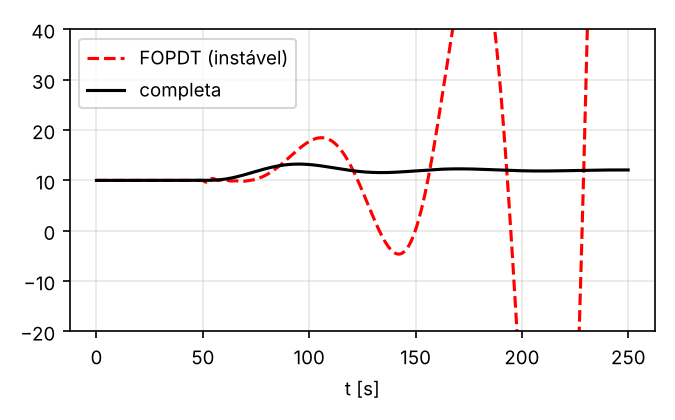
\includegraphics[width=.5\textwidth]{figs/i41_unst.png}\caption{O mesmo PID aplicado à FOPDT (instável) e à FT completa.}\end{figure}
\begin{just}A sintonia de Z--N foi \emph{projetada} para uma planta real em que se mediu $K_{cu}$ e $T_u$; o modelo FOPDT, ao trocar 3 polos por 1 polo e atraso, tem margem de ganho menor, então a sintonia que é estável na planta completa torna a FOPDT instável. Os parâmetros de Z--N só são válidos com $K_{cu}$ e $T_u$ da planta real. A resposta tem sobressinal grande (62\,\% do degrau), característico da razão 1/4; o SC chega a tocar o limite inferior no primeiro retorno, o que na bancada produzirá saturação e leve diferença em relação à simulação linear.\end{just}
\begin{todo}(i) Teste de ganho final: apenas $K_p$ ($K_i=K_d=0$), aumentar até oscilação sustentada, anotar $K_{cu}$ e $T_u$ (esperado: Figura do teste acima); (ii) recalcular os parâmetros com as fórmulas acima e implementar $K_p$, $K_i$, $K_d$, $\mu=0{,}1$; (iii) degrau de SP 10 $\to$ 12\,\%, gravar SO, SP, VP; (iv) confrontar VP e SC com a figura de simulação acima. Resultados: \underline{\hspace{6cm}}\end{todo}

%------------------------------------------------------------------
\section{Resumo dos controladores (para o OpenPLC)}
\begin{center}\small
\begin{tabular}{lccccc}\toprule Sintonia & $K_p$ & $T_i$ [s] & $T_d$ [s] & $K_i=K_p/T_i$ & $K_d=K_pT_d$\\\midrule
1.1 Dahlin ($\tau_c=40$ s) & 3,523 & 90,99 & 11,11 & 0,03872 & 39,15\\
2.1 PI\_D2GL (regulatório $\tau_c=20$ s, $\alpha=0{,}64$) & 5,057 & 90,99 & 11,11 & 0,05558 & 56,21\\
3.1 IAE ponto fixo (7-2.3) & 7,222 & 111,98 & 9,92 & 0,06449 & 71,63\\
4.1 Ziegler--Nichols (7-1.1) & 28,65 & 43,03 & 6,885 & 0,6659 & 197,3\\\bottomrule\end{tabular}\end{center}
Todos com $\mu=0{,}1$ (filtro derivativo $\mu T_d$), derivada na VP, $T_i$ e $T_d$ em segundos e $K_p$ em \%SC/\%VP.

\section{Conclusões}
\begin{itemize}
\item As FTs completas, deduzidas das equações dos nós com os $R$ e $C$ medidos, têm três polos reais ($\tau=68{,}7$; $16{,}0$; $10{,}4$ s) e reproduzem o degrau experimental com RMS de 0,7--1,7\,\% do degrau.
\item $\Vc1$ é curva tipo C ($\tau=23{,}3$ s, sem atraso); $\Vc2$ e $\Vc3$ são tipo S (Smith: $\Vc3$: $K=0{,}392$, $\tau=78{,}0$ s, $t_0=25{,}9$ s).
\item A FOPDT mantém a margem de fase da malha aberta (diferenças de até $6^\circ$ para $K_c\le5$) e subestima a margem de ganho (é conservadora). Por isso as sintonias dos itens 1.1, 2.1 e 3.1 são calculadas com a FOPDT (como pede o enunciado), enquanto $K_{cu}$ e $T_u$ do item 4.1 devem vir da planta real.
\item Os quatro controladores foram simulados (VP e SC, FOPDT e FT completa); as comparações com o experimento, VP e SC, serão feitas após os ensaios na bancada (assim como os itens 1.2, 1.3, 2.2 e 4.2).
\end{itemize}

\end{document}
